\documentclass{article}

% Packages
\usepackage{amsmath}
\usepackage{amsfonts}
\usepackage{amssymb}
\usepackage{geometry}
\usepackage{tikz}
\usepackage{float}
\usepackage{enumitem}
\usepackage{mathtools}
\usepackage{subcaption}
\usepackage[colorlinks=true]{hyperref}
% \usetikzlibrary{automata, arrows.meta, positioning,shapes}

\numberwithin{equation}{subsection}
\renewcommand{\thesubsection}{\thesection.\arabic{subsection}}
\renewcommand{\thesubsubsection}{\Alph{subsubsection}}

\newcommand{\setsubsubsectionnumber}[1]{\setcounter{subsubsection}{#1}\addtocounter{subsubsection}{-1}}

\DeclareMathOperator{\putx}{put}

\makeatletter
\newcommand{\leqnomode}{\tagsleft@true}
\newcommand{\reqnomode}{\tagsleft@false}
\makeatother

\newcommand{\abs}[1]{\vert #1\vert}
\newcommand{\tab}[1][30pt]{\hspace*{#1}}
\newcommand{\bracket}[1]{\biggl[#1\biggr]}


\title{Automata Homework 2}
\author{Ali Abbasi -- 98105879}
\begin{document}
\maketitle
\tableofcontents
\pagebreak

\section{Description of Automata and Concepts of Regular Languages}
\subsection{}
\subsubsection{}
We want to design an automaton that recognizes the language of strings over \(\{0, 1\}\) that their binary representation's remainder in division by \(5\) is \(2\).\\
Assume that we have an automaton that string \(s\) ends up in the state \(k\), if remainder of the binary representation of \(s\) in division by \(5\) is \(k\).
Now we derive the transition function of this automaton.
Assume that after reading the string \(s\), the next character is \(a\).
So our new string is \(s\circ a\). 
We can calculate the remainder of this new string divided by \(5\) as follows:
\begin{align}
s\circ a \mod 5 &= s\circ 0 + a \mod 5\\
&= 2s + a \mod 5\\
&= 2k + a \mod 5\\
\end{align}
Where \(k\) is the remainder of \(s\) in division by \(5\).
So we have:
\begin{align}
\delta(k, a) &= 2k + a \mod 5
\end{align}
The DFA for this automaton is shown in Figure~\ref{fig:automata1-1-1}.
\begin{figure}[H]
\centering
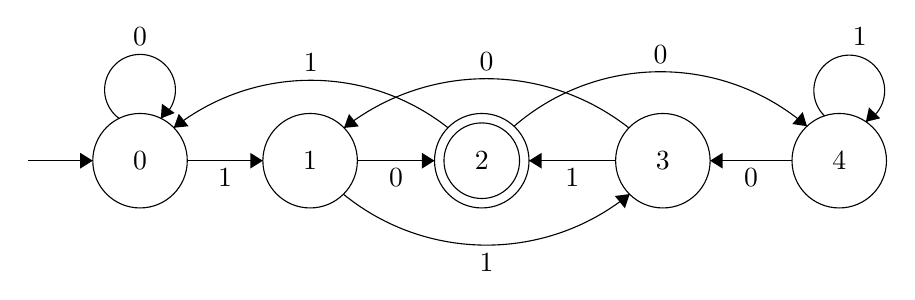
\begin{tikzpicture}[scale=0.2]
    \tikzstyle{every node}+=[inner sep=0pt]
    \draw [black] (7.3,-9.1) circle (3);
    \draw (7.3,-9.1) node {$0$};
    \draw [black] (18.1,-9.1) circle (3);
    \draw (18.1,-9.1) node {$1$};
    \draw [black] (29,-9.1) circle (3);
    \draw (29,-9.1) node {$2$};
    \draw [black] (29,-9.1) circle (2.4);
    \draw [black] (40.5,-9.1) circle (3);
    \draw (40.5,-9.1) node {$3$};
    \draw [black] (51.7,-9.1) circle (3);
    \draw (51.7,-9.1) node {$4$};
    \draw [black] (0.2,-9.1) -- (4.3,-9.1);
    \fill [black] (4.3,-9.1) -- (3.5,-8.6) -- (3.5,-9.6);
    \draw [black] (10.3,-9.1) -- (15.1,-9.1);
    \fill [black] (15.1,-9.1) -- (14.3,-8.6) -- (14.3,-9.6);
    \draw (12.7,-9.6) node [below] {$1$};
    \draw [black] (5.977,-6.42) arc (234:-54:2.25);
    \draw (7.3,-1.85) node [above] {$0$};
    \fill [black] (8.62,-6.42) -- (9.5,-6.07) -- (8.69,-5.48);
    \draw [black] (21.1,-9.1) -- (26,-9.1);
    \fill [black] (26,-9.1) -- (25.2,-8.6) -- (25.2,-9.6);
    \draw (23.55,-9.6) node [below] {$0$};
    \draw [black] (38.389,-11.224) arc (-50.79924:-129.20076:14.381);
    \fill [black] (38.39,-11.22) -- (37.45,-11.34) -- (38.09,-12.12);
    \draw (29.3,-14.96) node [below] {$1$};
    \draw [black] (31.047,-6.914) arc (130.84532:49.15468:14.225);
    \fill [black] (49.65,-6.91) -- (49.38,-6.01) -- (48.72,-6.77);
    \draw (40.35,-2.95) node [above] {$0$};
    \draw [black] (9.443,-7.008) arc (128.20556:51.79444:14.079);
    \fill [black] (9.44,-7.01) -- (10.38,-6.91) -- (9.76,-6.12);
    \draw (18.15,-3.49) node [above] {$1$};
    \draw [black] (37.5,-9.1) -- (32,-9.1);
    \fill [black] (32,-9.1) -- (32.8,-9.6) -- (32.8,-8.6);
    \draw (34.75,-9.6) node [below] {$1$};
    \draw [black] (20.254,-7.019) arc (128.14528:51.85472:14.646);
    \fill [black] (20.25,-7.02) -- (21.19,-6.92) -- (20.57,-6.13);
    \draw (29.3,-3.39) node [above] {$0$};
    \draw [black] (48.7,-9.1) -- (43.5,-9.1);
    \fill [black] (43.5,-9.1) -- (44.3,-9.6) -- (44.3,-8.6);
    \draw (46.1,-9.6) node [below] {$0$};
    \draw [black] (50.77,-6.26) arc (225.8699:-62.1301:2.25);
    \draw (53,-1.82) node [above] {$1$};
    \fill [black] (53.39,-6.63) -- (54.3,-6.41) -- (53.59,-5.71);
    \end{tikzpicture}
\caption{DFA describing the language.}
\label{fig:automata1-1-1}
\end{figure}

\subsubsection{}
First we design the NFA that recognizes the language of all strings with minimum size of 4 over the alphabet $\{a,b\}$ that their first and second to last letters are different.
The NFA is shown in Figure~\ref{fig:automata1-1-2-a}.
\begin{figure}[H]
\centering
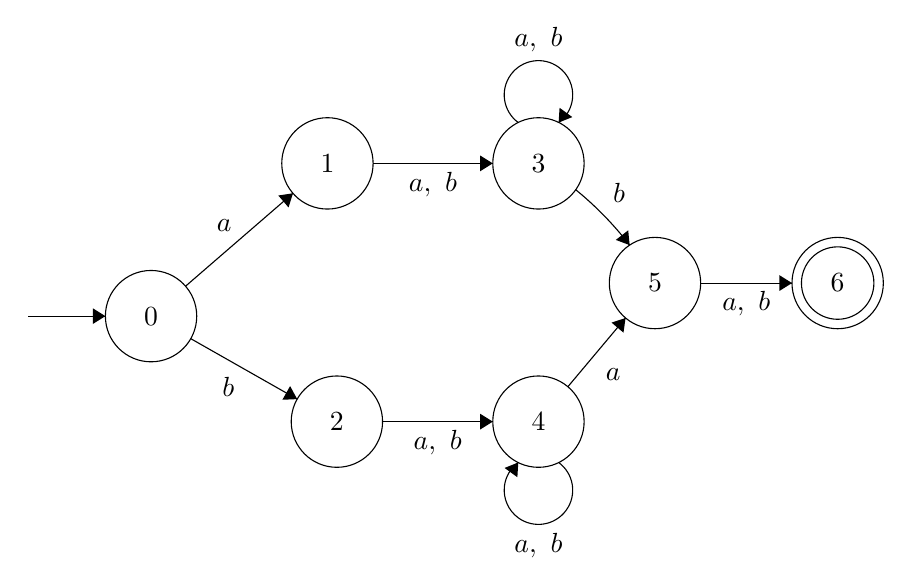
\begin{tikzpicture}[scale=0.2]
    \tikzstyle{every node}+=[inner sep=0pt]
    \draw [black] (8,-18.6) circle (2.9);
    \draw (8,-18.6) node {$0$};
    \draw [black] (32.6,-8.9) circle (2.9);
    \draw (32.6,-8.9) node {$3$};
    \draw [black] (32.6,-25.3) circle (2.9);
    \draw (32.6,-25.3) node {$4$};
    \draw [black] (40,-16.5) circle (2.9);
    \draw (40,-16.5) node {$5$};
    \draw [black] (51.6,-16.5) circle (2.9);
    \draw (51.6,-16.5) node {$6$};
    \draw [black] (51.6,-16.5) circle (2.3);
    \draw [black] (19.2,-8.9) circle (2.9);
    \draw (19.2,-8.9) node {$1$};
    \draw [black] (19.8,-25.3) circle (2.9);
    \draw (19.8,-25.3) node {$2$};
    \draw [black] (0.2,-18.6) -- (5.1,-18.6);
    \fill [black] (5.1,-18.6) -- (4.3,-18.1) -- (4.3,-19.1);
    \draw [black] (31.322,-6.31) arc (234:-54:2.175);
    \draw (32.6,-1.88) node [above] {$a,\mbox{ }b$};
    \fill [black] (33.88,-6.31) -- (34.75,-5.96) -- (33.94,-5.37);
    \draw [black] (34.966,-10.573) arc (50.8467:37.6255:21.322);
    \fill [black] (38.39,-14.09) -- (38.3,-13.15) -- (37.51,-13.76);
    \draw (37.31,-10.76) node [right] {$b$};
    \draw [black] (42.9,-16.5) -- (48.7,-16.5);
    \fill [black] (48.7,-16.5) -- (47.9,-16) -- (47.9,-17);
    \draw (45.8,-17) node [below] {$a,\mbox{ }b$};
    \draw [black] (34.47,-23.08) -- (38.13,-18.72);
    \fill [black] (38.13,-18.72) -- (37.24,-19.01) -- (38,-19.65);
    \draw (36.85,-22.34) node [right] {$a$};
    \draw [black] (33.878,-27.89) arc (54:-234:2.175);
    \draw (32.6,-32.33) node [below] {$a,\mbox{ }b$};
    \fill [black] (31.32,-27.89) -- (30.45,-28.24) -- (31.26,-28.83);
    \draw [black] (10.19,-16.7) -- (17.01,-10.8);
    \fill [black] (17.01,-10.8) -- (16.08,-10.94) -- (16.73,-11.7);
    \draw (12.65,-13.26) node [above] {$a$};
    \draw [black] (10.52,-20.03) -- (17.28,-23.87);
    \fill [black] (17.28,-23.87) -- (16.83,-23.04) -- (16.34,-23.91);
    \draw (12.9,-22.45) node [below] {$b$};
    \draw [black] (22.1,-8.9) -- (29.7,-8.9);
    \fill [black] (29.7,-8.9) -- (28.9,-8.4) -- (28.9,-9.4);
    \draw (25.9,-9.4) node [below] {$a,\mbox{ }b$};
    \draw [black] (22.7,-25.3) -- (29.7,-25.3);
    \fill [black] (29.7,-25.3) -- (28.9,-24.8) -- (28.9,-25.8);
    \draw (26.2,-25.8) node [below] {$a,\mbox{ }b$};
    \end{tikzpicture}
\caption{NFA describing the language.}
\label{fig:automata1-1-2-a}
\end{figure}
The NFA first gets \(a\) or \(b\) and gets one or more arbitrary characters.
When it reaches to the last two characters, it expects to get a different character than the first two characters.
Then it gets another arbitrary character and accept state is reached.
Note that state \(1\) and \(2\) are introduced only to make the minimum length of strings in this language 4.\\
Then we convert the NFA to an equivalent DFA using the subset construction algorithm.
The DFA is shown in Figure~\ref{fig:automata1-1-2-b}.
\begin{figure}[H]
\centering
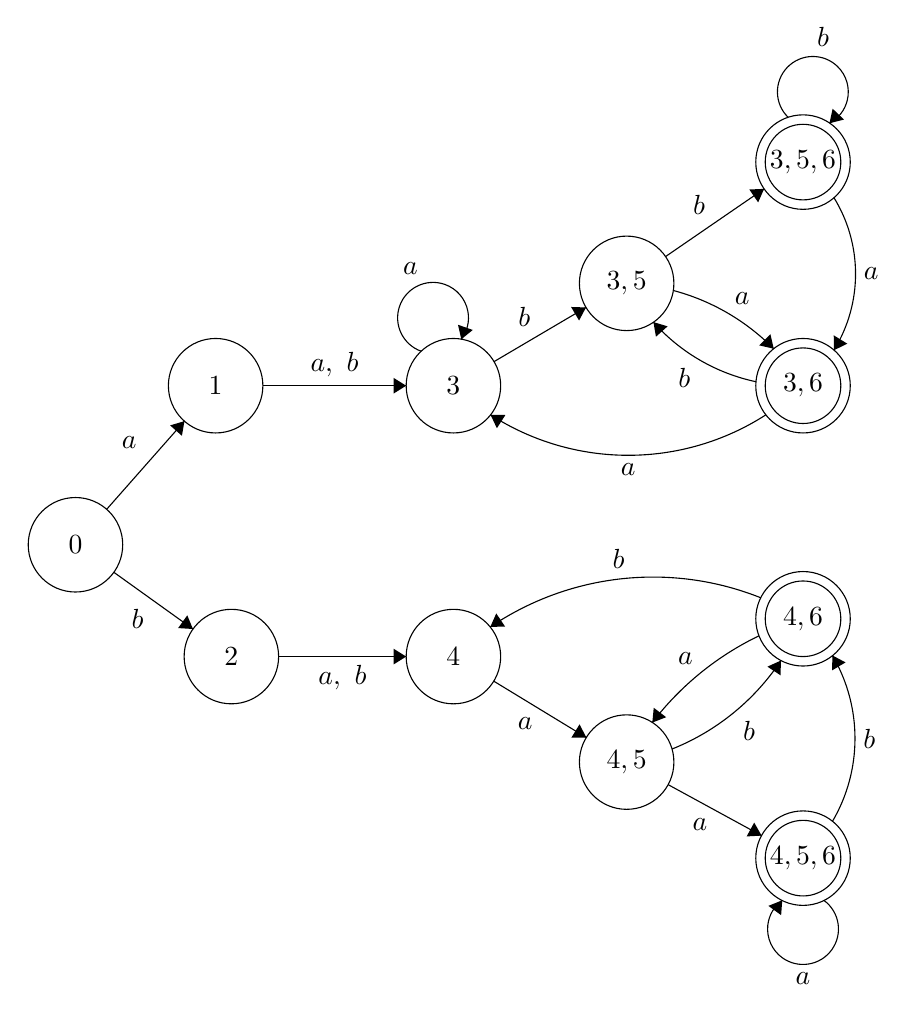
\begin{tikzpicture}[scale=0.2]
    \tikzstyle{every node}+=[inner sep=0pt]
    \draw [black] (3.3,-30.6) circle (3);
    \draw (3.3,-30.6) node {$0$};
    \draw [black] (12.2,-20.5) circle (3);
    \draw (12.2,-20.5) node {$1$};
    \draw [black] (13.2,-37.7) circle (3);
    \draw (13.2,-37.7) node {$2$};
    \draw [black] (27.3,-20.5) circle (3);
    \draw (27.3,-20.5) node {$3$};
    \draw [black] (27.3,-37.7) circle (3);
    \draw (27.3,-37.7) node {$4$};
    \draw [black] (38.3,-14) circle (3);
    \draw (38.3,-14) node {$3,5$};
    \draw [black] (49.5,-20.5) circle (3);
    \draw (49.5,-20.5) node {$3,6$};
    \draw [black] (49.5,-20.5) circle (2.4);
    \draw [black] (49.5,-6.3) circle (3);
    \draw (49.5,-6.3) node {$3,5,6$};
    \draw [black] (49.5,-6.3) circle (2.4);
    \draw [black] (38.3,-44.4) circle (3);
    \draw (38.3,-44.4) node {$4,5$};
    \draw [black] (49.5,-35.3) circle (3);
    \draw (49.5,-35.3) node {$4,6$};
    \draw [black] (49.5,-35.3) circle (2.4);
    \draw [black] (49.5,-50.5) circle (3);
    \draw (49.5,-50.5) node {$4,5,6$};
    \draw [black] (49.5,-50.5) circle (2.4);
    \draw [black] (5.28,-28.35) -- (10.22,-22.75);
    \fill [black] (10.22,-22.75) -- (9.31,-23.02) -- (10.06,-23.68);
    \draw (7.21,-24.1) node [left] {$a$};
    \draw [black] (5.74,-32.35) -- (10.76,-35.95);
    \fill [black] (10.76,-35.95) -- (10.4,-35.08) -- (9.82,-35.89);
    \draw (7.25,-34.65) node [below] {$b$};
    \draw [black] (15.2,-20.5) -- (24.3,-20.5);
    \fill [black] (24.3,-20.5) -- (23.5,-20) -- (23.5,-21);
    \draw (19.75,-20) node [above] {$a,\mbox{ }b$};
    \draw [black] (16.2,-37.7) -- (24.3,-37.7);
    \fill [black] (24.3,-37.7) -- (23.5,-37.2) -- (23.5,-38.2);
    \draw (20.25,-38.2) node [below] {$a,\mbox{ }b$};
    \draw [black] (29.88,-18.97) -- (35.72,-15.53);
    \fill [black] (35.72,-15.53) -- (34.77,-15.5) -- (35.28,-16.36);
    \draw (31.8,-16.75) node [above] {$b$};
    \draw [black] (25.263,-18.313) arc (250.69924:-37.30076:2.25);
    \draw (24.57,-13.49) node [above] {$a$};
    \fill [black] (27.8,-17.55) -- (28.53,-16.96) -- (27.59,-16.63);
    \draw [black] (40.77,-12.3) -- (47.03,-8);
    \fill [black] (47.03,-8) -- (46.09,-8.04) -- (46.65,-8.86);
    \draw (42.9,-9.65) node [above] {$b$};
    \draw [black] (41.26,-14.453) arc (75.1607:44.58121:13.984);
    \fill [black] (47.64,-18.15) -- (47.43,-17.23) -- (46.72,-17.94);
    \draw (45.64,-15.37) node [above] {$a$};
    \draw [black] (47.143,-22.348) arc (-57.22115:-122.77885:16.148);
    \fill [black] (29.66,-22.35) -- (30.06,-23.2) -- (30.6,-22.36);
    \draw (38.4,-25.42) node [below] {$a$};
    \draw [black] (46.518,-20.248) arc (-101.94361:-138.31447:12.078);
    \fill [black] (40,-16.46) -- (40.16,-17.39) -- (40.9,-16.73);
    \draw (41.96,-19.38) node [below] {$b$};
    \draw [black] (51.46,-8.554) arc (31.68588:-31.68588:9.226);
    \fill [black] (51.46,-18.25) -- (52.31,-17.83) -- (51.45,-17.3);
    \draw (53.33,-13.4) node [right] {$a$};
    \draw [black] (48.562,-3.463) arc (226.03002:-61.96998:2.25);
    \draw (50.77,0.98) node [above] {$b$};
    \fill [black] (51.18,-3.83) -- (52.1,-3.6) -- (51.38,-2.91);
    \draw [black] (29.86,-39.26) -- (35.74,-42.84);
    \fill [black] (35.74,-42.84) -- (35.31,-42) -- (34.79,-42.85);
    \draw (31.86,-41.55) node [below] {$a$};
    \draw [black] (48.101,-37.948) arc (-33.59292:-68.21936:14.985);
    \fill [black] (48.1,-37.95) -- (47.24,-38.34) -- (48.07,-38.89);
    \draw (46.07,-41.78) node [below] {$b$};
    \draw [black] (39.93,-41.885) arc (142.49196:115.69575:18.836);
    \fill [black] (39.93,-41.89) -- (40.81,-41.55) -- (40.02,-40.95);
    \draw (42.04,-38.24) node [above] {$a$};
    \draw [black] (29.636,-35.823) arc (124.11572:68.22463:18.437);
    \fill [black] (29.64,-35.82) -- (30.58,-35.79) -- (30.02,-34.96);
    \draw (37.78,-32.17) node [above] {$b$};
    \draw [black] (40.93,-45.83) -- (46.87,-49.07);
    \fill [black] (46.87,-49.07) -- (46.4,-48.24) -- (45.92,-49.12);
    \draw (42.96,-47.95) node [below] {$a$};
    \draw [black] (50.823,-53.18) arc (54:-234:2.25);
    \draw (49.5,-57.75) node [below] {$a$};
    \fill [black] (48.18,-53.18) -- (47.3,-53.53) -- (48.11,-54.12);
    \draw [black] (51.368,-37.634) arc (30.41677:-30.41677:10.402);
    \fill [black] (51.37,-37.63) -- (51.34,-38.58) -- (52.2,-38.07);
    \draw (53.3,-42.9) node [right] {$b$};
    \end{tikzpicture}
\caption{The Equivalent DFA describing the language.}
\label{fig:automata1-1-2-b}
\end{figure}

\subsection{}
\(D\) possibly has multiple accept states.
DFA \(D'\) will have the same structure as \(D\), and accept states that are subset of the those of \(D\).
Think of DFA \(D\) as a graph with states as nodes and transitions as edges.
If an accept state in \(D\) (for example \(f_1\)), has a path to another accept state (\(f_2\)), then for all \(w\) accepted via \(f_1\), there is a non-empty string \(x\) such that \(w x\) is accepted via \(f_2\).
In this case we remove \(f_1\) from the accept states of \(D'\).
Using DFAs notation, we have:
\begin{align}
D &= (Q, \Sigma, \delta, q_0, F)\\
\implies D' &= (Q, \Sigma, \delta, q_0, F')\\
\text{where } F' &= \left\{f \in F | \forall f' \in F, \text{ there is no path from } f \text{ to } f' \right\}
\end{align}

\subsection{}
\subsubsection{}
\begin{align}
\begin{rcases*}
g\circ f (q_{0,1}) = g (q_{0,2}) = q_{0,3} \\
g\circ f(\delta_1 (q, a)) = g(\delta_2(f(q), a)) = \delta_3(g\circ f(q), a)
\end{rcases*} \implies g\circ f: Q_1\to Q_3 \text{ is a morphism.}
\end{align}

\subsubsection{}
We prove this by induction on the length of the string.
Suppose \(w=w_1w_2\cdots w_n\).
We have:\\
\textbf{Base Case:} \(n=1\):\\
\begin{align}
h(\delta_1(q, w_1)) &= \delta_2(h(q), w_1)
\end{align}
\textbf{Induction Hypothesis:} Suppose it holds for \(n=k\). Then:
\begin{align}
w_{1:k} &\triangleq w_1w_2\cdots w_k\\
h(\delta_1^*(q, w_{1:k})) &= \delta_2^*(h(q), w_{1:k})
\end{align}
\textbf{Inductive Step:}
\begin{align}
h(\delta_1^*(q, w_{1:k+1})) &= h(\delta_1(\delta_1^*(q, w_{1:k}), w_{k+1}))\\
&= \delta_2(h(\delta_1^*(q, w_{1:k})), w_{k+1})\\
&= \delta_2(\delta_2^*(h(q), w_{1:k}), w_{k+1}) & (\text{Induction Hypothesis})\\
&= \delta_2^*(h(q), w_{1:k+1})
\end{align}
So it holds for all \(w \in \Sigma^*\) with length \(n>0\)
(Note that \(\delta(q, \epsilon)\) is undefined for DFA).

\section{Equivalence and Minimization}
\subsection{}
\begin{table}[H]
\centering
\begin{tabular}{c|c|c}
q & \(\delta(q, a)\) & \(\delta(q, b)\)\\
\hline
01 & 234 & \(\emptyset\)\\
234 & 014 & 0134\\
014 & 234 & \(\emptyset\)\\
0134 & 01234 & 014\\
01234 & 01234 & 0134\\
\(\emptyset\) & \(\emptyset\) & \(\emptyset\)
\end{tabular}
\caption{States and transition functions of the equivalent DFA}
\end{table}
Each state of the DFA is a subset of NFA's states.
And if it contains the accept state of NFA (4), it is an accept state of DFA.
Introducing new names for brevity:
\begin{table}[H]
\centering
\begin{tabular}{c|c|c}
q & \(\delta(q, a)\) & \(\delta(q, b)\)\\
\hline
A & B & F\\
B & C & D\\
C & B & F\\
D & E & C\\
E & E & D\\
F & F & F
\end{tabular}
\caption{States and transition functions of the DFA}
\end{table}
\begin{figure}[H]
\centering
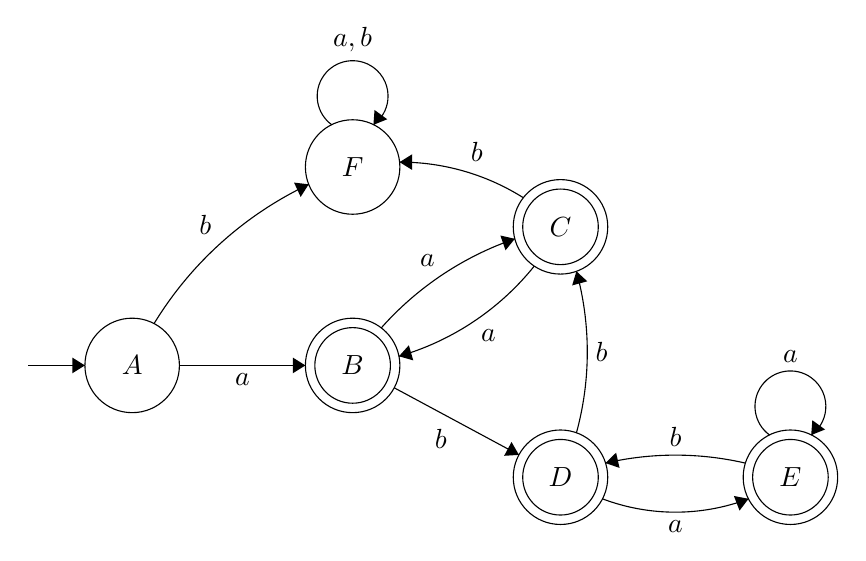
\begin{tikzpicture}[scale=0.2]
    \tikzstyle{every node}+=[inner sep=0pt]
    \draw [black] (6.8,-21.7) circle (3);
    \draw (6.8,-21.7) node {$A$};
    \draw [black] (20.8,-21.7) circle (3);
    \draw (20.8,-21.7) node {$B$};
    \draw [black] (20.8,-21.7) circle (2.4);
    \draw [black] (34,-12.9) circle (3);
    \draw (34,-12.9) node {$C$};
    \draw [black] (34,-12.9) circle (2.4);
    \draw [black] (34,-28.8) circle (3);
    \draw (34,-28.8) node {$D$};
    \draw [black] (34,-28.8) circle (2.4);
    \draw [black] (48.6,-28.8) circle (3);
    \draw (48.6,-28.8) node {$E$};
    \draw [black] (48.6,-28.8) circle (2.4);
    \draw [black] (20.8,-9.1) circle (3);
    \draw (20.8,-9.1) node {$F$};
    \draw [black] (9.8,-21.7) -- (17.8,-21.7);
    \fill [black] (17.8,-21.7) -- (17,-21.2) -- (17,-22.2);
    \draw (13.8,-22.2) node [below] {$a$};
    \draw [black] (22.618,-19.317) arc (138.3883:108.99183:20.092);
    \fill [black] (31.1,-13.66) -- (30.18,-13.45) -- (30.51,-14.39);
    \draw (25.55,-15.44) node [above] {$a$};
    \draw [black] (32.335,-15.391) arc (-38.77189:-73.84798:17.141);
    \fill [black] (23.74,-21.12) -- (24.65,-21.38) -- (24.37,-20.42);
    \draw (29.42,-19.42) node [below] {$a$};
    \draw [black] (23.44,-23.12) -- (31.36,-27.38);
    \fill [black] (31.36,-27.38) -- (30.89,-26.56) -- (30.42,-27.44);
    \draw (26.4,-25.75) node [below] {$b$};
    \draw [black] (35.012,-15.721) arc (15.30311:-15.30311:19.433);
    \fill [black] (35.01,-15.72) -- (34.74,-16.62) -- (35.7,-16.36);
    \draw (36.2,-20.85) node [right] {$b$};
    \draw [black] (45.939,-30.171) arc (-69.29128:-110.70872:13.119);
    \fill [black] (45.94,-30.17) -- (45.01,-29.99) -- (45.37,-30.92);
    \draw (41.3,-31.52) node [below] {$a$};
    \draw [black] (47.277,-26.12) arc (234:-54:2.25);
    \draw (48.6,-21.55) node [above] {$a$};
    \fill [black] (49.92,-26.12) -- (50.8,-25.77) -- (49.99,-25.18);
    \draw [black] (36.86,-27.903) arc (103.03985:76.96015:19.679);
    \fill [black] (36.86,-27.9) -- (37.75,-28.21) -- (37.53,-27.24);
    \draw (41.3,-26.9) node [above] {$b$};
    \draw [black] (0.2,-21.7) -- (3.8,-21.7);
    \fill [black] (3.8,-21.7) -- (3,-21.2) -- (3,-22.2);
    \draw [black] (8.191,-19.044) arc (148.63415:115.34027:23.064);
    \fill [black] (18.01,-10.2) -- (17.08,-10.09) -- (17.5,-11);
    \draw (11.44,-13.42) node [above] {$b$};
    \draw [black] (19.477,-6.42) arc (234:-54:2.25);
    \draw (20.8,-1.85) node [above] {$a,b$};
    \fill [black] (22.12,-6.42) -- (23,-6.07) -- (22.19,-5.48);
    \draw [black] (23.779,-8.789) arc (90.11096:57.76906:14.692);
    \fill [black] (23.78,-8.79) -- (24.58,-9.29) -- (24.58,-8.29);
    \draw (28.68,-8.81) node [above] {$b$};
    \end{tikzpicture}
\caption{The Equivalent DFA.}
\label{fig:automata2-1}
\end{figure}

\subsection{}
Note that both accept states of DFA are unreachable!
So we can remove them and the transitions to them.
And the Hopcroft algorithm ends in the first step, since all remaining states are in one class.
So the minimized DFA is a single non-accept state.
\begin{figure}[H]
\centering
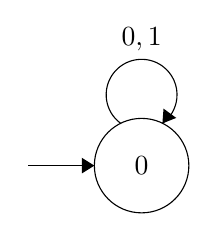
\begin{tikzpicture}[scale=0.2]
    \tikzstyle{every node}+=[inner sep=0pt]
    \draw [black] (7.4,-9) circle (3);
    \draw (7.4,-9) node {$0$};
    \draw [black] (0.2,-9) -- (4.4,-9);
    \fill [black] (4.4,-9) -- (3.6,-8.5) -- (3.6,-9.5);
    \draw [black] (6.077,-6.32) arc (234:-54:2.25);
    \draw (7.4,-1.75) node [above] {$0, 1$};
    \fill [black] (8.72,-6.32) -- (9.6,-5.97) -- (8.79,-5.38);
    \end{tikzpicture}
\caption{The minimized DFA!}
\label{fig:automata2-2}
\end{figure}

\section{Regular Expressions and Grammars}
\subsection{}
\subsubsection{}
First we design DFA describing \((a\cup b)^*\) language using the rules we learned.
Then we simplify it with removing extra \(\epsilon\) transitions (Figure~\ref{fig:automata3-1-a}).
\begin{figure}[H]
\centering
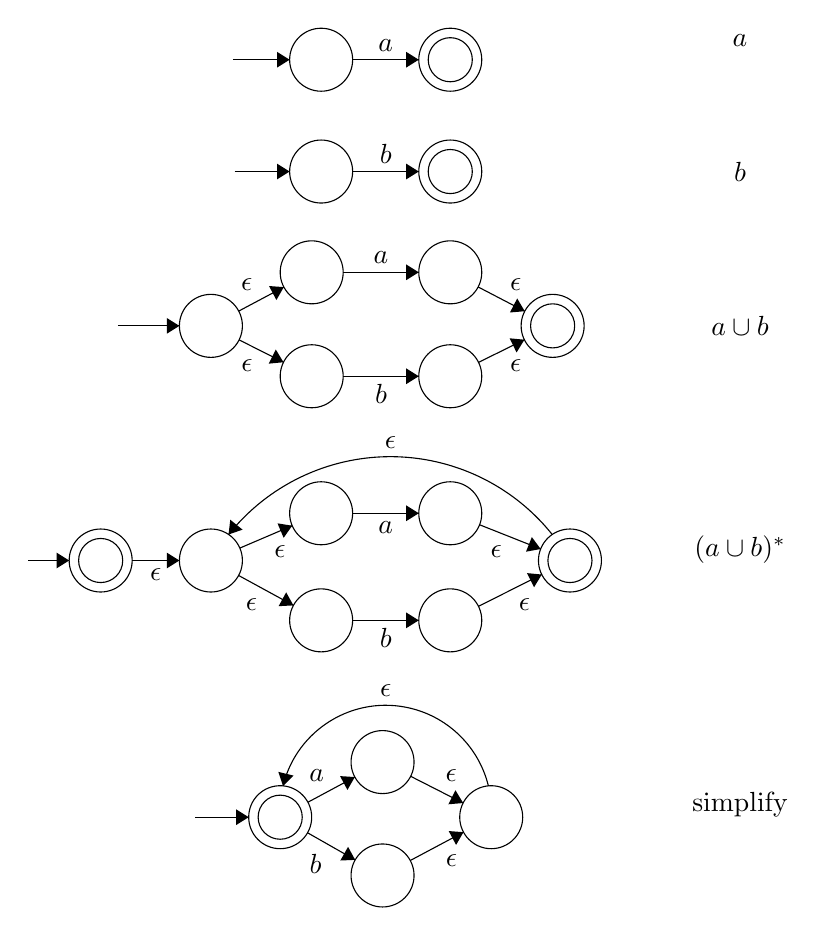
\begin{tikzpicture}[scale=0.2]
    \tikzstyle{every node}+=[inner sep=0pt]
    \draw [black] (18.8,-2.2) circle (2);
    \draw [black] (27,-2.2) circle (2);
    \draw [black] (27,-2.2) circle (1.4);
    \draw [black] (18.8,-9.3) circle (2);
    \draw [black] (27,-9.3) circle (2);
    \draw [black] (27,-9.3) circle (1.4);
    \draw (45.4,-1) node {$a$};
    \draw (45.4,-9.3) node {$b$};
    \draw [black] (11.8,-19.1) circle (2);
    \draw [black] (18.2,-15.7) circle (2);
    \draw [black] (18.2,-22.3) circle (2);
    \draw [black] (27,-15.7) circle (2);
    \draw [black] (27,-22.3) circle (2);
    \draw [black] (33.5,-19.1) circle (2);
    \draw [black] (33.5,-19.1) circle (1.4);
    \draw (45.4,-19.1) node {$a\cup b$};
    \draw [black] (18.8,-31) circle (2);
    \draw [black] (27,-31) circle (2);
    \draw [black] (18.8,-37.8) circle (2);
    \draw [black] (27,-37.8) circle (2);
    \draw [black] (34.6,-34) circle (2);
    \draw [black] (34.6,-34) circle (1.4);
    \draw [black] (11.8,-34) circle (2);
    \draw [black] (4.8,-34) circle (2);
    \draw [black] (4.8,-34) circle (1.4);
    \draw (45.4,-33.3) node {$(a\cup b)^*$};
    \draw [black] (16.2,-50.3) circle (2);
    \draw [black] (16.2,-50.3) circle (1.4);
    \draw [black] (22.7,-46.8) circle (2);
    \draw [black] (22.7,-54) circle (2);
    \draw [black] (29.6,-50.3) circle (2);
    \draw (45.4,-49.5) node {simplify};
    \draw [black] (20.8,-2.2) -- (25,-2.2);
    \fill [black] (25,-2.2) -- (24.2,-1.7) -- (24.2,-2.7);
    \draw (22.9,-1.7) node [above] {$a$};
    \draw [black] (13.2,-2.2) -- (16.8,-2.2);
    \fill [black] (16.8,-2.2) -- (16,-1.7) -- (16,-2.7);
    \draw [black] (20.8,-9.3) -- (25,-9.3);
    \fill [black] (25,-9.3) -- (24.2,-8.8) -- (24.2,-9.8);
    \draw (22.9,-8.8) node [above] {$b$};
    \draw [black] (13.3,-9.3) -- (16.8,-9.3);
    \fill [black] (16.8,-9.3) -- (16,-8.8) -- (16,-9.8);
    \draw [black] (13.57,-18.16) -- (16.43,-16.64);
    \fill [black] (16.43,-16.64) -- (15.49,-16.57) -- (15.96,-17.46);
    \draw (14.08,-16.9) node [above] {$\epsilon$};
    \draw [black] (13.59,-19.99) -- (16.41,-21.41);
    \fill [black] (16.41,-21.41) -- (15.92,-20.6) -- (15.47,-21.5);
    \draw (14.09,-21.2) node [below] {$\epsilon$};
    \draw [black] (5.9,-19.1) -- (9.8,-19.1);
    \fill [black] (9.8,-19.1) -- (9,-18.6) -- (9,-19.6);
    \draw [black] (20.2,-15.7) -- (25,-15.7);
    \fill [black] (25,-15.7) -- (24.2,-15.2) -- (24.2,-16.2);
    \draw (22.6,-15.2) node [above] {$a$};
    \draw [black] (20.2,-22.3) -- (25,-22.3);
    \fill [black] (25,-22.3) -- (24.2,-21.8) -- (24.2,-22.8);
    \draw (22.6,-22.8) node [below] {$b$};
    \draw [black] (28.77,-16.63) -- (31.73,-18.17);
    \fill [black] (31.73,-18.17) -- (31.25,-17.36) -- (30.79,-18.25);
    \draw (31.16,-16.9) node [above] {$\epsilon$};
    \draw [black] (28.79,-21.42) -- (31.71,-19.98);
    \fill [black] (31.71,-19.98) -- (30.77,-19.89) -- (31.21,-20.79);
    \draw (31.16,-21.2) node [below] {$\epsilon$};
    \draw [black] (20.8,-31) -- (25,-31);
    \fill [black] (25,-31) -- (24.2,-30.5) -- (24.2,-31.5);
    \draw (22.9,-31.5) node [below] {$a$};
    \draw [black] (20.8,-37.8) -- (25,-37.8);
    \fill [black] (25,-37.8) -- (24.2,-37.3) -- (24.2,-38.3);
    \draw (22.9,-38.3) node [below] {$b$};
    \draw [black] (28.86,-31.73) -- (32.74,-33.27);
    \fill [black] (32.74,-33.27) -- (32.18,-32.51) -- (31.81,-33.44);
    \draw (29.92,-33.02) node [below] {$\epsilon$};
    \draw [black] (28.79,-36.91) -- (32.81,-34.89);
    \fill [black] (32.81,-34.89) -- (31.87,-34.8) -- (32.32,-35.7);
    \draw (31.71,-36.4) node [below] {$\epsilon$};
    \draw [black] (0.2,-34) -- (2.8,-34);
    \fill [black] (2.8,-34) -- (2,-33.5) -- (2,-34.5);
    \draw [black] (6.8,-34) -- (9.8,-34);
    \fill [black] (9.8,-34) -- (9,-33.5) -- (9,-34.5);
    \draw (8.3,-34.5) node [below] {$\epsilon$};
    \draw [black] (13.64,-33.21) -- (16.96,-31.79);
    \fill [black] (16.96,-31.79) -- (16.03,-31.64) -- (16.42,-32.56);
    \draw (16.19,-33.01) node [below] {$\epsilon$};
    \draw [black] (13.56,-34.95) -- (17.04,-36.85);
    \fill [black] (17.04,-36.85) -- (16.58,-36.02) -- (16.1,-36.9);
    \draw (14.38,-36.4) node [below] {$\epsilon$};
    \draw [black] (12.925,-32.349) arc (141.38267:38.61733:13.151);
    \fill [black] (12.92,-32.35) -- (13.81,-32.04) -- (13.03,-31.41);
    \draw (23.2,-26.91) node [above] {$\epsilon$};
    \draw [black] (10.8,-50.3) -- (14.2,-50.3);
    \fill [black] (14.2,-50.3) -- (13.4,-49.8) -- (13.4,-50.8);
    \draw [black] (17.96,-49.35) -- (20.94,-47.75);
    \fill [black] (20.94,-47.75) -- (20,-47.69) -- (20.47,-48.57);
    \draw (18.51,-48.05) node [above] {$a$};
    \draw [black] (17.94,-51.29) -- (20.96,-53.01);
    \fill [black] (20.96,-53.01) -- (20.51,-52.18) -- (20.02,-53.05);
    \draw (18.45,-52.65) node [below] {$b$};
    \draw [black] (24.48,-47.7) -- (27.82,-49.4);
    \fill [black] (27.82,-49.4) -- (27.33,-48.59) -- (26.88,-49.48);
    \draw (27.06,-48.05) node [above] {$\epsilon$};
    \draw [black] (24.46,-53.05) -- (27.84,-51.25);
    \fill [black] (27.84,-51.25) -- (26.9,-51.18) -- (27.37,-52.06);
    \draw (27.07,-52.65) node [below] {$\epsilon$};
    \draw [black] (16.379,-48.315) arc (-193.70504:-346.29496:6.712);
    \fill [black] (16.38,-48.32) -- (17.05,-47.66) -- (16.08,-47.42);
    \draw (22.9,-42.69) node [above] {$\epsilon$};
    \end{tikzpicture}
\caption{DFA for \((a\cup b)^*\).}
\label{fig:automata3-1-a}
\end{figure}
Now we design DFA for \((a\cup b)^*(a\cup ba)^*a(b\cup ab)^*\) in the same way (Figure~\ref{fig:automata3-1-b}).
\begin{figure}[H]
\centering
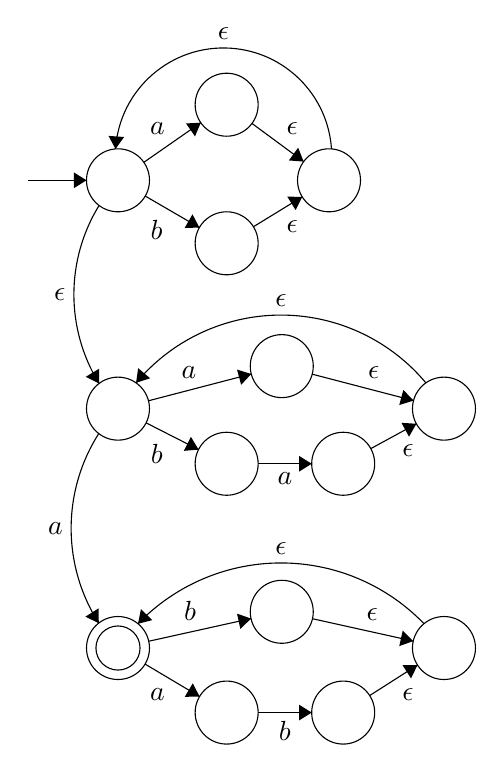
\begin{tikzpicture}[scale=0.2]
    \tikzstyle{every node}+=[inner sep=0pt]
    \draw [black] (5.9,-10.3) circle (2);
    \draw [black] (12.8,-5.5) circle (2);
    \draw [black] (12.8,-14.3) circle (2);
    \draw [black] (19.3,-10.3) circle (2);
    \draw [black] (16.3,-22.1) circle (2);
    \draw [black] (5.9,-24.8) circle (2);
    \draw [black] (12.8,-28.3) circle (2);
    \draw [black] (20.2,-28.3) circle (2);
    \draw [black] (26.6,-24.8) circle (2);
    \draw [black] (5.9,-40) circle (2);
    \draw [black] (5.9,-40) circle (1.4);
    \draw [black] (16.3,-37.7) circle (2);
    \draw [black] (26.6,-40) circle (2);
    \draw [black] (12.8,-44.1) circle (2);
    \draw [black] (20.2,-44.1) circle (2);
    \draw [black] (7.54,-9.16) -- (11.16,-6.64);
    \fill [black] (11.16,-6.64) -- (10.22,-6.69) -- (10.79,-7.51);
    \draw (8.4,-7.4) node [above] {$a$};
    \draw [black] (7.63,-11.3) -- (11.07,-13.3);
    \fill [black] (11.07,-13.3) -- (10.63,-12.46) -- (10.13,-13.33);
    \draw (8.35,-12.8) node [below] {$b$};
    \draw [black] (14.41,-6.69) -- (17.69,-9.11);
    \fill [black] (17.69,-9.11) -- (17.34,-8.23) -- (16.75,-9.04);
    \draw (16.97,-7.4) node [above] {$\epsilon$};
    \draw [black] (14.5,-13.25) -- (17.6,-11.35);
    \fill [black] (17.6,-11.35) -- (16.65,-11.34) -- (17.18,-12.19);
    \draw (16.97,-12.8) node [below] {$\epsilon$};
    \draw [black] (5.743,-8.313) arc (-183.8075:-356.1925:6.873);
    \fill [black] (5.74,-8.31) -- (6.29,-7.55) -- (5.3,-7.48);
    \draw (12.6,-1.4) node [above] {$\epsilon$};
    \draw [black] (0.2,-10.3) -- (3.9,-10.3);
    \fill [black] (3.9,-10.3) -- (3.1,-9.8) -- (3.1,-10.8);
    \draw [black] (7.84,-24.3) -- (14.36,-22.6);
    \fill [black] (14.36,-22.6) -- (13.46,-22.32) -- (13.72,-23.29);
    \draw (10.4,-22.89) node [above] {$a$};
    \draw [black] (7.68,-25.7) -- (11.02,-27.4);
    \fill [black] (11.02,-27.4) -- (10.53,-26.59) -- (10.08,-27.48);
    \draw (8.36,-27.05) node [below] {$b$};
    \draw [black] (14.8,-28.3) -- (18.2,-28.3);
    \fill [black] (18.2,-28.3) -- (17.4,-27.8) -- (17.4,-28.8);
    \draw (16.5,-28.8) node [below] {$a$};
    \draw [black] (18.23,-22.61) -- (24.67,-24.29);
    \fill [black] (24.67,-24.29) -- (24.02,-23.61) -- (23.76,-24.57);
    \draw (22.14,-22.89) node [above] {$\epsilon$};
    \draw [black] (21.95,-27.34) -- (24.85,-25.76);
    \fill [black] (24.85,-25.76) -- (23.9,-25.7) -- (24.38,-26.58);
    \draw (24.32,-27.05) node [below] {$\epsilon$};
    \draw [black] (7.048,-23.165) arc (140.15887:39.84113:11.985);
    \fill [black] (7.05,-23.16) -- (7.94,-22.87) -- (7.18,-22.23);
    \draw (16.25,-18.36) node [above] {$\epsilon$};
    \draw [black] (4.7,-23.204) arc (-148.37871:-211.62129:10.783);
    \fill [black] (4.7,-23.2) -- (4.71,-22.26) -- (3.85,-22.78);
    \draw (2.6,-17.55) node [left] {$\epsilon$};
    \draw [black] (7.85,-39.57) -- (14.35,-38.13);
    \fill [black] (14.35,-38.13) -- (13.46,-37.82) -- (13.67,-38.79);
    \draw (10.47,-38.27) node [above] {$b$};
    \draw [black] (18.25,-38.14) -- (24.65,-39.56);
    \fill [black] (24.65,-39.56) -- (23.98,-38.9) -- (23.76,-39.88);
    \draw (22.04,-38.28) node [above] {$\epsilon$};
    \draw [black] (7.62,-41.02) -- (11.08,-43.08);
    \fill [black] (11.08,-43.08) -- (10.65,-42.24) -- (10.14,-43.1);
    \draw (8.41,-42.55) node [below] {$a$};
    \draw [black] (14.8,-44.1) -- (18.2,-44.1);
    \fill [black] (18.2,-44.1) -- (17.4,-43.6) -- (17.4,-44.6);
    \draw (16.5,-44.6) node [below] {$b$};
    \draw [black] (21.88,-43.02) -- (24.92,-41.08);
    \fill [black] (24.92,-41.08) -- (23.97,-41.09) -- (24.51,-41.93);
    \draw (24.32,-42.55) node [below] {$\epsilon$};
    \draw [black] (7.169,-38.457) arc (136.03147:43.96853:12.618);
    \fill [black] (7.17,-38.46) -- (8.08,-38.23) -- (7.36,-37.53);
    \draw (16.25,-34.1) node [above] {$\epsilon$};
    \draw [black] (4.68,-38.419) arc (-147.47253:-212.52747:11.193);
    \fill [black] (4.68,-38.42) -- (4.67,-37.48) -- (3.83,-38.01);
    \draw (2.42,-32.4) node [left] {$a$};
    \end{tikzpicture}
\caption{DFA for \((a\cup b)^*(a\cup ba)^*a(b\cup ab)^*\).}
\label{fig:automata3-1-b}
\end{figure}

\subsubsection{}
Using the same method as last part, we derive the following DFA for this language (Figure~\ref{fig:automata3-1-c}).
\begin{figure}[H]
\centering
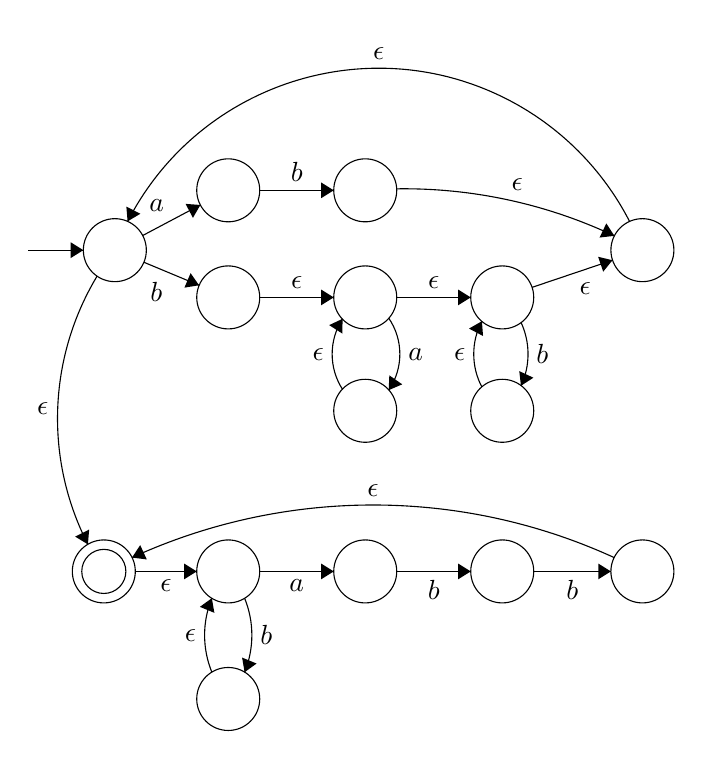
\begin{tikzpicture}[scale=0.2]
    \tikzstyle{every node}+=[inner sep=0pt]
    \draw [black] (5.7,-11.8) circle (2);
    \draw [black] (12.9,-8) circle (2);
    \draw [black] (12.9,-14.8) circle (2);
    \draw [black] (21.6,-8) circle (2);
    \draw [black] (21.6,-14.8) circle (2);
    \draw [black] (21.6,-22) circle (2);
    \draw [black] (30.3,-14.8) circle (2);
    \draw [black] (30.3,-22) circle (2);
    \draw [black] (39.2,-11.8) circle (2);
    \draw [black] (5,-32.2) circle (2);
    \draw [black] (5,-32.2) circle (1.4);
    \draw [black] (12.9,-32.2) circle (2);
    \draw [black] (12.9,-40.3) circle (2);
    \draw [black] (21.6,-32.2) circle (2);
    \draw [black] (30.3,-32.2) circle (2);
    \draw [black] (39.2,-32.2) circle (2);
    \draw [black] (0.2,-11.8) -- (3.7,-11.8);
    \fill [black] (3.7,-11.8) -- (2.9,-11.3) -- (2.9,-12.3);
    \draw [black] (7.47,-10.87) -- (11.13,-8.93);
    \fill [black] (11.13,-8.93) -- (10.19,-8.86) -- (10.66,-9.75);
    \draw (8.36,-9.4) node [above] {$a$};
    \draw [black] (7.55,-12.57) -- (11.05,-14.03);
    \fill [black] (11.05,-14.03) -- (10.51,-13.26) -- (10.12,-14.18);
    \draw (8.33,-13.81) node [below] {$b$};
    \draw [black] (14.9,-8) -- (19.6,-8);
    \fill [black] (19.6,-8) -- (18.8,-7.5) -- (18.8,-8.5);
    \draw (17.25,-7.5) node [above] {$b$};
    \draw [black] (14.9,-14.8) -- (19.6,-14.8);
    \fill [black] (19.6,-14.8) -- (18.8,-14.3) -- (18.8,-15.3);
    \draw (17.25,-14.3) node [above] {$\epsilon$};
    \draw [black] (23.086,-16.108) arc (34.50537:-34.50537:4.047);
    \fill [black] (23.09,-20.69) -- (23.95,-20.32) -- (23.13,-19.75);
    \draw (24.3,-18.4) node [right] {$a$};
    \draw [black] (20.159,-20.641) arc (-147.18925:-212.81075:4.135);
    \fill [black] (20.16,-16.16) -- (19.31,-16.56) -- (20.15,-17.1);
    \draw (19,-18.4) node [left] {$\epsilon$};
    \draw [black] (23.6,-14.8) -- (28.3,-14.8);
    \fill [black] (28.3,-14.8) -- (27.5,-14.3) -- (27.5,-15.3);
    \draw (25.95,-14.3) node [above] {$\epsilon$};
    \draw [black] (31.493,-16.387) arc (24.93044:-24.93044:4.775);
    \fill [black] (31.49,-20.41) -- (32.28,-19.9) -- (31.38,-19.48);
    \draw (32.44,-18.4) node [right] {$b$};
    \draw [black] (29.009,-20.494) arc (-152.1641:-207.8359:4.485);
    \fill [black] (29.01,-16.31) -- (28.19,-16.78) -- (29.08,-17.25);
    \draw (27.99,-18.4) node [left] {$\epsilon$};
    \draw [black] (23.597,-7.906) arc (90.87443:64.75825:31.293);
    \fill [black] (37.42,-10.89) -- (36.91,-10.1) -- (36.48,-11);
    \draw (31.25,-8.03) node [above] {$\epsilon$};
    \draw [black] (32.2,-14.16) -- (37.3,-12.44);
    \fill [black] (37.3,-12.44) -- (36.39,-12.22) -- (36.71,-13.17);
    \draw (35.57,-13.83) node [below] {$\epsilon$};
    \draw [black] (6.514,-9.974) arc (152.78749:27.21251:17.92);
    \fill [black] (6.51,-9.97) -- (7.32,-9.49) -- (6.43,-9.03);
    \draw (22.45,0.25) node [above] {$\epsilon$};
    \draw [black] (3.988,-30.476) arc (-152.85689:-211.07363:17.51);
    \fill [black] (3.99,-30.48) -- (4.07,-29.54) -- (3.18,-29.99);
    \draw (1.52,-21.88) node [left] {$\epsilon$};
    \draw [black] (7,-32.2) -- (10.9,-32.2);
    \fill [black] (10.9,-32.2) -- (10.1,-31.7) -- (10.1,-32.7);
    \draw (8.95,-32.7) node [below] {$\epsilon$};
    \draw [black] (13.939,-33.899) arc (22.21891:-22.21891:6.217);
    \fill [black] (13.94,-38.6) -- (14.7,-38.05) -- (13.78,-37.67);
    \draw (14.9,-36.25) node [right] {$b$};
    \draw [black] (11.861,-38.601) arc (-157.78109:-202.21891:6.217);
    \fill [black] (11.86,-33.9) -- (11.1,-34.45) -- (12.02,-34.83);
    \draw (10.9,-36.25) node [left] {$\epsilon$};
    \draw [black] (23.6,-32.2) -- (28.3,-32.2);
    \fill [black] (28.3,-32.2) -- (27.5,-31.7) -- (27.5,-32.7);
    \draw (25.95,-32.7) node [below] {$b$};
    \draw [black] (14.9,-32.2) -- (19.6,-32.2);
    \fill [black] (19.6,-32.2) -- (18.8,-31.7) -- (18.8,-32.7);
    \draw (17.25,-32.7) node [below] {$a$};
    \draw [black] (32.3,-32.2) -- (37.2,-32.2);
    \fill [black] (37.2,-32.2) -- (36.4,-31.7) -- (36.4,-32.7);
    \draw (34.75,-32.7) node [below] {$b$};
    \draw [black] (6.795,-31.318) arc (114.5976:65.4024:36.769);
    \fill [black] (6.79,-31.32) -- (7.73,-31.44) -- (7.31,-30.53);
    \draw (22.1,-27.48) node [above] {$\epsilon$};
    \end{tikzpicture}
\caption{DFA for \((ab\cup ba^*b^*)^*(b^*abb)^*\).}
\label{fig:automata3-1-c}
\end{figure}

\subsection{}
\subsubsection{}
First we convert the DFA to GNFA.
Then we rip the GNFA states one by one, to get the regular expression (Figure~\ref{fig:automata3-2-1}).\\
Note that to avoid overcrowding the figure, we do not draw the arrows with \(\emptyset\) labels.
\begin{figure}
\centering  
\begin{subfigure}[b]{\textwidth}
\centering
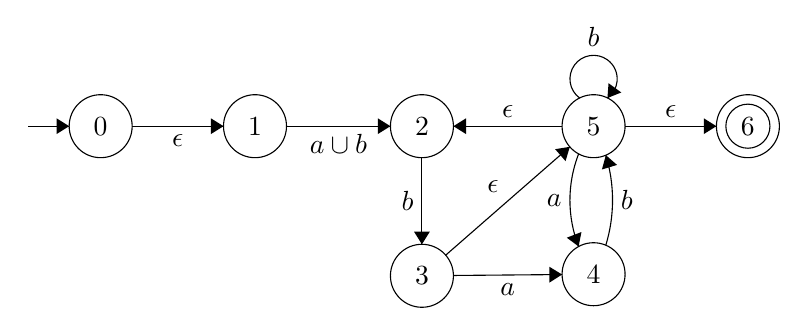
\begin{tikzpicture}[scale=0.2]
    \tikzstyle{every node}+=[inner sep=0pt]
    \draw [black] (4.8,-6.9) circle (2);
    \draw (4.8,-6.9) node {$0$};
    \draw [black] (14.6,-6.9) circle (2);
    \draw (14.6,-6.9) node {$1$};
    \draw [black] (25.2,-6.9) circle (2);
    \draw (25.2,-6.9) node {$2$};
    \draw [black] (25.2,-16.4) circle (2);
    \draw (25.2,-16.4) node {$3$};
    \draw [black] (36.1,-16.3) circle (2);
    \draw (36.1,-16.3) node {$4$};
    \draw [black] (36.1,-6.9) circle (2);
    \draw (36.1,-6.9) node {$5$};
    \draw [black] (45.9,-6.9) circle (2);
    \draw (45.9,-6.9) node {$6$};
    \draw [black] (45.9,-6.9) circle (1.4);
    \draw [black] (0.2,-6.9) -- (2.8,-6.9);
    \fill [black] (2.8,-6.9) -- (2,-6.4) -- (2,-7.4);
    \draw [black] (6.8,-6.9) -- (12.6,-6.9);
    \fill [black] (12.6,-6.9) -- (11.8,-6.4) -- (11.8,-7.4);
    \draw (9.7,-7.4) node [below] {$\epsilon$};
    \draw [black] (16.6,-6.9) -- (23.2,-6.9);
    \fill [black] (23.2,-6.9) -- (22.4,-6.4) -- (22.4,-7.4);
    \draw (19.9,-7.4) node [below] {$a\cup b$};
    \draw [black] (25.2,-8.9) -- (25.2,-14.4);
    \fill [black] (25.2,-14.4) -- (25.7,-13.6) -- (24.7,-13.6);
    \draw (24.7,-11.65) node [left] {$b$};
    \draw [black] (27.2,-16.38) -- (34.1,-16.32);
    \fill [black] (34.1,-16.32) -- (33.3,-15.83) -- (33.3,-16.83);
    \draw (30.65,-16.86) node [below] {$a$};
    \draw [black] (34.1,-6.9) -- (27.2,-6.9);
    \fill [black] (27.2,-6.9) -- (28,-7.4) -- (28,-6.4);
    \draw (30.65,-6.4) node [above] {$\epsilon$};
    \draw [black] (26.71,-15.09) -- (34.59,-8.21);
    \fill [black] (34.59,-8.21) -- (33.66,-8.36) -- (34.32,-9.12);
    \draw (29.72,-11.16) node [above] {$\epsilon$};
    \draw [black] (38.1,-6.9) -- (43.9,-6.9);
    \fill [black] (43.9,-6.9) -- (43.1,-6.4) -- (43.1,-7.4);
    \draw (41,-6.4) node [above] {$\epsilon$};
    \draw [black] (35.218,-5.114) arc (234:-54:1.5);
    \draw (36.1,-1.9) node [above] {$b$};
    \fill [black] (36.98,-5.11) -- (37.86,-4.76) -- (37.05,-4.17);
    \draw [black] (35.152,-14.545) arc (-158.68732:-201.31268:8.102);
    \fill [black] (35.15,-14.54) -- (35.33,-13.62) -- (34.4,-13.98);
    \draw (34.1,-11.6) node [left] {$a$};
    \draw [black] (36.876,-8.739) arc (17.02346:-17.02346:9.771);
    \fill [black] (36.88,-8.74) -- (36.63,-9.65) -- (37.59,-9.36);
    \draw (37.8,-11.6) node [right] {$b$};
    \end{tikzpicture}
\subcaption{The initial GNFA.}
\end{subfigure}

\medskip
\begin{subfigure}[b]{\textwidth}
\centering
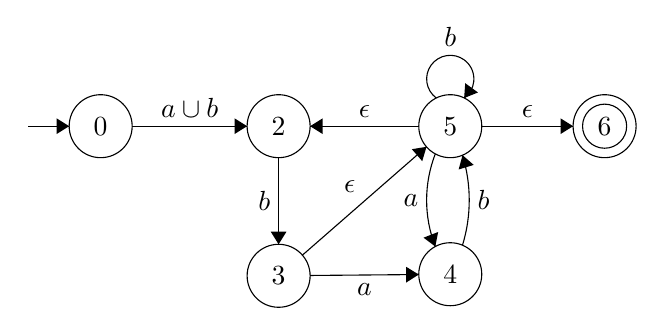
\begin{tikzpicture}[scale=0.2]
    \tikzstyle{every node}+=[inner sep=0pt]
    \draw [black] (4.8,-6.9) circle (2);
    \draw (4.8,-6.9) node {$0$};
    \draw [black] (16.1,-6.9) circle (2);
    \draw (16.1,-6.9) node {$2$};
    \draw [black] (16.1,-16.4) circle (2);
    \draw (16.1,-16.4) node {$3$};
    \draw [black] (27,-16.3) circle (2);
    \draw (27,-16.3) node {$4$};
    \draw [black] (27,-6.9) circle (2);
    \draw (27,-6.9) node {$5$};
    \draw [black] (36.8,-6.9) circle (2);
    \draw (36.8,-6.9) node {$6$};
    \draw [black] (36.8,-6.9) circle (1.4);
    \draw [black] (0.2,-6.9) -- (2.8,-6.9);
    \fill [black] (2.8,-6.9) -- (2,-6.4) -- (2,-7.4);
    \draw [black] (16.1,-8.9) -- (16.1,-14.4);
    \fill [black] (16.1,-14.4) -- (16.6,-13.6) -- (15.6,-13.6);
    \draw (15.6,-11.65) node [left] {$b$};
    \draw [black] (18.1,-16.38) -- (25,-16.32);
    \fill [black] (25,-16.32) -- (24.2,-15.83) -- (24.2,-16.83);
    \draw (21.55,-16.86) node [below] {$a$};
    \draw [black] (25,-6.9) -- (18.1,-6.9);
    \fill [black] (18.1,-6.9) -- (18.9,-7.4) -- (18.9,-6.4);
    \draw (21.55,-6.4) node [above] {$\epsilon$};
    \draw [black] (17.61,-15.09) -- (25.49,-8.21);
    \fill [black] (25.49,-8.21) -- (24.56,-8.36) -- (25.22,-9.12);
    \draw (20.62,-11.16) node [above] {$\epsilon$};
    \draw [black] (29,-6.9) -- (34.8,-6.9);
    \fill [black] (34.8,-6.9) -- (34,-6.4) -- (34,-7.4);
    \draw (31.9,-6.4) node [above] {$\epsilon$};
    \draw [black] (26.118,-5.114) arc (234:-54:1.5);
    \draw (27,-1.9) node [above] {$b$};
    \fill [black] (27.88,-5.11) -- (28.76,-4.76) -- (27.95,-4.17);
    \draw [black] (26.052,-14.545) arc (-158.68732:-201.31268:8.102);
    \fill [black] (26.05,-14.54) -- (26.23,-13.62) -- (25.3,-13.98);
    \draw (25,-11.6) node [left] {$a$};
    \draw [black] (27.776,-8.739) arc (17.02346:-17.02346:9.771);
    \fill [black] (27.78,-8.74) -- (27.53,-9.65) -- (28.49,-9.36);
    \draw (28.7,-11.6) node [right] {$b$};
    \draw [black] (6.8,-6.9) -- (14.1,-6.9);
    \fill [black] (14.1,-6.9) -- (13.3,-6.4) -- (13.3,-7.4);
    \draw (10.45,-6.4) node [above] {$a\cup b$};
    \end{tikzpicture}
\subcaption{After ripping \(1\).}
\end{subfigure}

\medskip
\begin{subfigure}[b]{\textwidth}
\centering
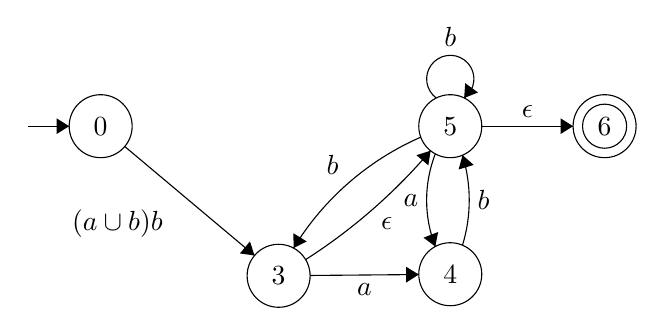
\begin{tikzpicture}[scale=0.2]
    \tikzstyle{every node}+=[inner sep=0pt]
    \draw [black] (4.8,-6.9) circle (2);
    \draw (4.8,-6.9) node {$0$};
    \draw [black] (16.1,-16.4) circle (2);
    \draw (16.1,-16.4) node {$3$};
    \draw [black] (27,-16.3) circle (2);
    \draw (27,-16.3) node {$4$};
    \draw [black] (27,-6.9) circle (2);
    \draw (27,-6.9) node {$5$};
    \draw [black] (36.8,-6.9) circle (2);
    \draw (36.8,-6.9) node {$6$};
    \draw [black] (36.8,-6.9) circle (1.4);
    \draw [black] (0.2,-6.9) -- (2.8,-6.9);
    \fill [black] (2.8,-6.9) -- (2,-6.4) -- (2,-7.4);
    \draw [black] (18.1,-16.38) -- (25,-16.32);
    \fill [black] (25,-16.32) -- (24.2,-15.83) -- (24.2,-16.83);
    \draw (21.55,-16.86) node [below] {$a$};
    \draw [black] (25.747,-8.458) arc (-40.42411:-57.42771:35.584);
    \fill [black] (25.75,-8.46) -- (24.85,-8.74) -- (25.61,-9.39);
    \draw (22.97,-12.7) node [below] {$\epsilon$};
    \draw [black] (29,-6.9) -- (34.8,-6.9);
    \fill [black] (34.8,-6.9) -- (34,-6.4) -- (34,-7.4);
    \draw (31.9,-6.4) node [above] {$\epsilon$};
    \draw [black] (26.118,-5.114) arc (234:-54:1.5);
    \draw (27,-1.9) node [above] {$b$};
    \fill [black] (27.88,-5.11) -- (28.76,-4.76) -- (27.95,-4.17);
    \draw [black] (26.052,-14.545) arc (-158.68732:-201.31268:8.102);
    \fill [black] (26.05,-14.54) -- (26.23,-13.62) -- (25.3,-13.98);
    \draw (25,-11.6) node [left] {$a$};
    \draw [black] (27.776,-8.739) arc (17.02346:-17.02346:9.771);
    \fill [black] (27.78,-8.74) -- (27.53,-9.65) -- (28.49,-9.36);
    \draw (28.7,-11.6) node [right] {$b$};
    \draw [black] (17.047,-14.639) arc (148.53091:113.61727:17.864);
    \fill [black] (17.05,-14.64) -- (17.89,-14.22) -- (17.04,-13.7);
    \draw (19.53,-10.01) node [above] {$b$};
    \draw [black] (6.33,-8.19) -- (14.57,-15.11);
    \fill [black] (14.57,-15.11) -- (14.28,-14.22) -- (13.64,-14.98);
    \draw (5.86,-12.14) node [below] {$(a\cup b)b$};
    \end{tikzpicture}
\subcaption{After ripping \(2\).}
\end{subfigure}

\medskip
\begin{subfigure}[b]{\textwidth}
\centering
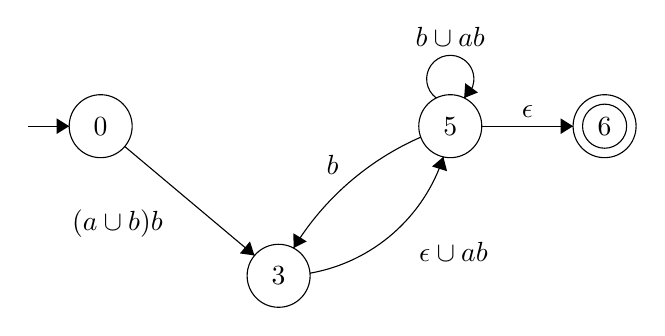
\begin{tikzpicture}[scale=0.2]
    \tikzstyle{every node}+=[inner sep=0pt]
    \draw [black] (4.8,-6.9) circle (2);
    \draw (4.8,-6.9) node {$0$};
    \draw [black] (16.1,-16.4) circle (2);
    \draw (16.1,-16.4) node {$3$};
    \draw [black] (27,-6.9) circle (2);
    \draw (27,-6.9) node {$5$};
    \draw [black] (36.8,-6.9) circle (2);
    \draw (36.8,-6.9) node {$6$};
    \draw [black] (36.8,-6.9) circle (1.4);
    \draw [black] (0.2,-6.9) -- (2.8,-6.9);
    \fill [black] (2.8,-6.9) -- (2,-6.4) -- (2,-7.4);
    \draw [black] (26.565,-8.849) arc (-17.84573:-80.00609:10.888);
    \fill [black] (26.56,-8.85) -- (25.84,-9.46) -- (26.8,-9.76);
    \draw (27.2,-14.21) node [below] {$\epsilon\cup ab$};
    \draw [black] (29,-6.9) -- (34.8,-6.9);
    \fill [black] (34.8,-6.9) -- (34,-6.4) -- (34,-7.4);
    \draw (31.9,-6.4) node [above] {$\epsilon$};
    \draw [black] (26.118,-5.114) arc (234:-54:1.5);
    \draw (27,-1.9) node [above] {$b\cup ab$};
    \fill [black] (27.88,-5.11) -- (28.76,-4.76) -- (27.95,-4.17);
    \draw [black] (17.047,-14.639) arc (148.53091:113.61727:17.864);
    \fill [black] (17.05,-14.64) -- (17.89,-14.22) -- (17.04,-13.7);
    \draw (19.53,-10.01) node [above] {$b$};
    \draw [black] (6.33,-8.19) -- (14.57,-15.11);
    \fill [black] (14.57,-15.11) -- (14.28,-14.22) -- (13.64,-14.98);
    \draw (5.86,-12.14) node [below] {$(a\cup b)b$};
    \end{tikzpicture}
\subcaption{After ripping \(4\).}
\end{subfigure}

\medskip
\caption{Converting DFA to Regular Expression.}
\label{fig:automata3-2-1}
\end{figure}%
\begin{figure}[t]\ContinuedFloat
\centering  
\begin{subfigure}[t]{\textwidth}
\centering
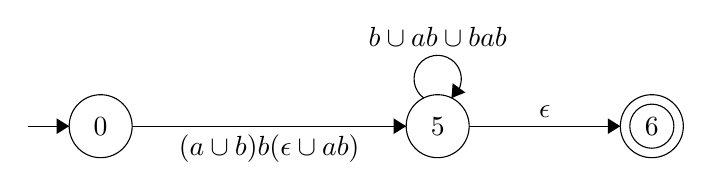
\begin{tikzpicture}[scale=0.2]
    \tikzstyle{every node}+=[inner sep=0pt]
    \draw [black] (4.8,-6.9) circle (2);
    \draw (4.8,-6.9) node {$0$};
    \draw [black] (26.2,-6.9) circle (2);
    \draw (26.2,-6.9) node {$5$};
    \draw [black] (39.8,-6.9) circle (2);
    \draw (39.8,-6.9) node {$6$};
    \draw [black] (39.8,-6.9) circle (1.4);
    \draw [black] (0.2,-6.9) -- (2.8,-6.9);
    \fill [black] (2.8,-6.9) -- (2,-6.4) -- (2,-7.4);
    \draw [black] (28.2,-6.9) -- (37.8,-6.9);
    \fill [black] (37.8,-6.9) -- (37,-6.4) -- (37,-7.4);
    \draw (33,-6.4) node [above] {$\epsilon$};
    \draw [black] (25.318,-5.114) arc (234:-54:1.5);
    \draw (26.2,-1.9) node [above] {$b\cup ab\cup bab$};
    \fill [black] (27.08,-5.11) -- (27.96,-4.76) -- (27.15,-4.17);
    \draw [black] (6.8,-6.9) -- (24.2,-6.9);
    \fill [black] (24.2,-6.9) -- (23.4,-6.4) -- (23.4,-7.4);
    \draw (15.5,-7.4) node [below] {$(a\cup b)b(\epsilon\cup ab)$};
    \end{tikzpicture}
\subcaption{After ripping \(3\) (\(b\cup ab \cup b(\epsilon \cup ab) = b\cup ab \cup bab\)).}
\end{subfigure}

\medskip
\begin{subfigure}[t]{\textwidth}
\centering
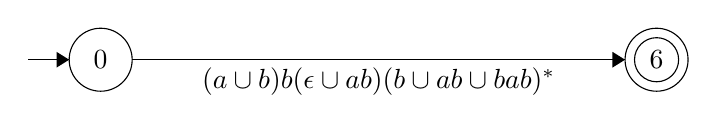
\begin{tikzpicture}[scale=0.2]
    \tikzstyle{every node}+=[inner sep=0pt]
    \draw [black] (4.8,-2.2) circle (2);
    \draw (4.8,-2.2) node {$0$};
    \draw [black] (40.1,-2.2) circle (2);
    \draw (40.1,-2.2) node {$6$};
    \draw [black] (40.1,-2.2) circle (1.4);
    \draw [black] (0.2,-2.2) -- (2.8,-2.2);
    \fill [black] (2.8,-2.2) -- (2,-1.7) -- (2,-2.7);
    \draw [black] (6.8,-2.2) -- (38.1,-2.2);
    \fill [black] (38.1,-2.2) -- (37.3,-1.7) -- (37.3,-2.7);
    \draw (22.45,-2.7) node [below] {$(a\cup b)b(\epsilon\cup ab)(b\cup ab \cup bab)^*$};
    \end{tikzpicture}
\subcaption{After ripping \(5\).}
\end{subfigure}

\medskip
\caption{Converting DFA to Regular Expression. (Continued)}
\end{figure}

\pagebreak
So the resulting regular expression is \((a\cup b)b(\epsilon\cup ab)(b\cup ab \cup bab)^*\).

\subsubsection{}
Using the same procedure as last part, we can get the corresponding regular expression (Figure~\ref{fig:automata3-2-2}).
\begin{figure}
\centering  
\begin{subfigure}[b]{\textwidth}
\centering
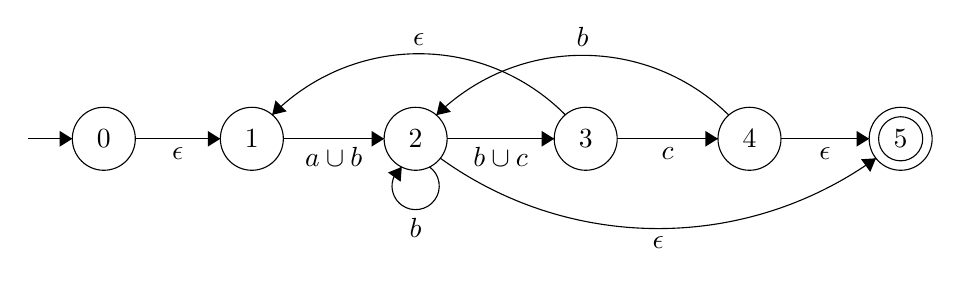
\begin{tikzpicture}[scale=0.2]
    \tikzstyle{every node}+=[inner sep=0pt]
    \draw [black] (5,-7.7) circle (2);
    \draw (5,-7.7) node {$0$};
    \draw [black] (14.4,-7.7) circle (2);
    \draw (14.4,-7.7) node {$1$};
    \draw [black] (24.8,-7.7) circle (2);
    \draw (24.8,-7.7) node {$2$};
    \draw [black] (35.6,-7.7) circle (2);
    \draw (35.6,-7.7) node {$3$};
    \draw [black] (46,-7.7) circle (2);
    \draw (46,-7.7) node {$4$};
    \draw [black] (55.6,-7.7) circle (2);
    \draw (55.6,-7.7) node {$5$};
    \draw [black] (55.6,-7.7) circle (1.4);
    \draw [black] (0.2,-7.7) -- (3,-7.7);
    \fill [black] (3,-7.7) -- (2.2,-7.2) -- (2.2,-8.2);
    \draw [black] (7,-7.7) -- (12.4,-7.7);
    \fill [black] (12.4,-7.7) -- (11.6,-7.2) -- (11.6,-8.2);
    \draw (9.7,-8.2) node [below] {$\epsilon$};
    \draw [black] (16.4,-7.7) -- (22.8,-7.7);
    \fill [black] (22.8,-7.7) -- (22,-7.2) -- (22,-8.2);
    \draw (19.6,-8.2) node [below] {$a\cup b$};
    \draw [black] (26.8,-7.7) -- (33.6,-7.7);
    \fill [black] (33.6,-7.7) -- (32.8,-7.2) -- (32.8,-8.2);
    \draw (30.2,-8.2) node [below] {$b\cup c$};
    \draw [black] (37.6,-7.7) -- (44,-7.7);
    \fill [black] (44,-7.7) -- (43.2,-7.2) -- (43.2,-8.2);
    \draw (40.8,-8.2) node [below] {$c$};
    \draw [black] (48,-7.7) -- (53.6,-7.7);
    \fill [black] (53.6,-7.7) -- (52.8,-7.2) -- (52.8,-8.2);
    \draw (50.8,-8.2) node [below] {$\epsilon$};
    \draw [black] (54.029,-8.937) arc (-54.20883:-125.79117:23.646);
    \fill [black] (54.03,-8.94) -- (53.09,-9) -- (53.67,-9.81);
    \draw (40.2,-13.9) node [below] {$\epsilon$};
    \draw [black] (25.682,-9.486) arc (54:-234:1.5);
    \draw (24.8,-12.7) node [below] {$b$};
    \fill [black] (23.92,-9.49) -- (23.04,-9.84) -- (23.85,-10.43);
    \draw [black] (26.116,-6.196) arc (134.48235:45.51765:13.25);
    \fill [black] (26.12,-6.2) -- (27.04,-5.99) -- (26.34,-5.28);
    \draw (35.4,-1.9) node [above] {$b$};
    \draw [black] (15.694,-6.178) arc (135.25835:44.74165:13.102);
    \fill [black] (15.69,-6.18) -- (16.61,-5.96) -- (15.9,-5.26);
    \draw (25,-1.8) node [above] {$\epsilon$};
    \end{tikzpicture}
\subcaption{The initial GNFA.}
\end{subfigure}

\medskip
\centering  
\begin{subfigure}[b]{\textwidth}
\centering
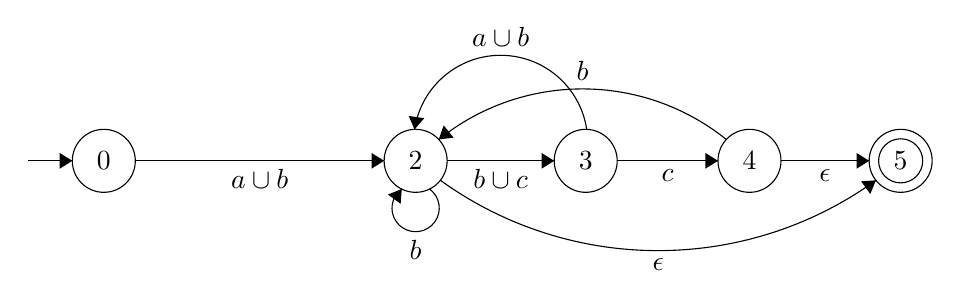
\begin{tikzpicture}[scale=0.2]
    \tikzstyle{every node}+=[inner sep=0pt]
    \draw [black] (5,-9.1) circle (2);
    \draw (5,-9.1) node {$0$};
    \draw [black] (24.8,-9.1) circle (2);
    \draw (24.8,-9.1) node {$2$};
    \draw [black] (35.6,-9.1) circle (2);
    \draw (35.6,-9.1) node {$3$};
    \draw [black] (46,-9.1) circle (2);
    \draw (46,-9.1) node {$4$};
    \draw [black] (55.6,-9.1) circle (2);
    \draw (55.6,-9.1) node {$5$};
    \draw [black] (55.6,-9.1) circle (1.4);
    \draw [black] (0.2,-9.1) -- (3,-9.1);
    \fill [black] (3,-9.1) -- (2.2,-8.6) -- (2.2,-9.6);
    \draw [black] (26.8,-9.1) -- (33.6,-9.1);
    \fill [black] (33.6,-9.1) -- (32.8,-8.6) -- (32.8,-9.6);
    \draw (30.2,-9.6) node [below] {$b\cup c$};
    \draw [black] (37.6,-9.1) -- (44,-9.1);
    \fill [black] (44,-9.1) -- (43.2,-8.6) -- (43.2,-9.6);
    \draw (40.8,-9.6) node [below] {$c$};
    \draw [black] (48,-9.1) -- (53.6,-9.1);
    \fill [black] (53.6,-9.1) -- (52.8,-8.6) -- (52.8,-9.6);
    \draw (50.8,-9.6) node [below] {$\epsilon$};
    \draw [black] (54.029,-10.337) arc (-54.20883:-125.79117:23.646);
    \fill [black] (54.03,-10.34) -- (53.09,-10.4) -- (53.67,-11.21);
    \draw (40.2,-15.3) node [below] {$\epsilon$};
    \draw [black] (25.682,-10.886) arc (54:-234:1.5);
    \draw (24.8,-14.1) node [below] {$b$};
    \fill [black] (23.92,-10.89) -- (23.04,-11.24) -- (23.85,-11.83);
    \draw [black] (26.269,-7.745) arc (128.76337:51.23663:14.584);
    \fill [black] (26.27,-7.74) -- (27.21,-7.63) -- (26.58,-6.85);
    \draw (35.4,-4.03) node [above] {$b$};
    \draw [black] (7,-9.1) -- (22.8,-9.1);
    \fill [black] (22.8,-9.1) -- (22,-8.6) -- (22,-9.6);
    \draw (14.9,-9.6) node [below] {$a\cup b$};
    \draw [black] (24.734,-7.112) arc (-188.45967:-351.54033:5.526);
    \fill [black] (24.73,-7.11) -- (25.35,-6.39) -- (24.36,-6.25);
    \draw (30.2,-1.9) node [above] {$a\cup b$};
\end{tikzpicture}
\subcaption{After ripping \(1\).}
\end{subfigure}

\medskip
\begin{subfigure}[b]{\textwidth}
\centering
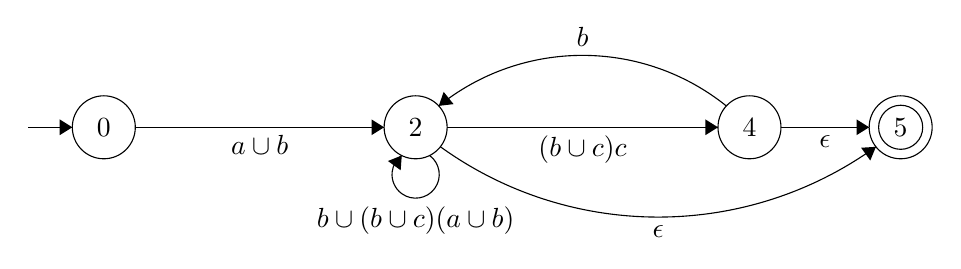
\begin{tikzpicture}[scale=0.2]
    \tikzstyle{every node}+=[inner sep=0pt]
    \draw [black] (5,-7) circle (2);
    \draw (5,-7) node {$0$};
    \draw [black] (24.8,-7) circle (2);
    \draw (24.8,-7) node {$2$};
    \draw [black] (46,-7) circle (2);
    \draw (46,-7) node {$4$};
    \draw [black] (55.6,-7) circle (2);
    \draw (55.6,-7) node {$5$};
    \draw [black] (55.6,-7) circle (1.4);
    \draw [black] (0.2,-7) -- (3,-7);
    \fill [black] (3,-7) -- (2.2,-6.5) -- (2.2,-7.5);
    \draw [black] (48,-7) -- (53.6,-7);
    \fill [black] (53.6,-7) -- (52.8,-6.5) -- (52.8,-7.5);
    \draw (50.8,-7.5) node [below] {$\epsilon$};
    \draw [black] (54.029,-8.237) arc (-54.20883:-125.79117:23.646);
    \fill [black] (54.03,-8.24) -- (53.09,-8.3) -- (53.67,-9.11);
    \draw (40.2,-13.2) node [below] {$\epsilon$};
    \draw [black] (25.682,-8.786) arc (54:-234:1.5);
    \draw (24.8,-12) node [below] {$b\cup (b\cup c)(a\cup b)$};
    \fill [black] (23.92,-8.79) -- (23.04,-9.14) -- (23.85,-9.73);
    \draw [black] (26.269,-5.645) arc (128.76337:51.23663:14.584);
    \fill [black] (26.27,-5.64) -- (27.21,-5.53) -- (26.58,-4.75);
    \draw (35.4,-1.93) node [above] {$b$};
    \draw [black] (7,-7) -- (22.8,-7);
    \fill [black] (22.8,-7) -- (22,-6.5) -- (22,-7.5);
    \draw (14.9,-7.5) node [below] {$a\cup b$};
    \draw [black] (26.8,-7) -- (44,-7);
    \fill [black] (44,-7) -- (43.2,-6.5) -- (43.2,-7.5);
    \draw (35.4,-7.5) node [below] {$(b\cup c)c$};
    \end{tikzpicture}
\subcaption{After ripping \(3\).}
\end{subfigure}

\medskip
\begin{subfigure}[b]{\textwidth}
\centering
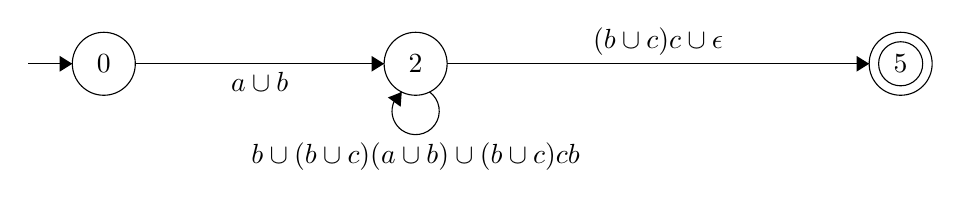
\begin{tikzpicture}[scale=0.2]
    \tikzstyle{every node}+=[inner sep=0pt]
    \draw [black] (5,-2.4) circle (2);
    \draw (5,-2.4) node {$0$};
    \draw [black] (24.8,-2.4) circle (2);
    \draw (24.8,-2.4) node {$2$};
    \draw [black] (55.6,-2.4) circle (2);
    \draw (55.6,-2.4) node {$5$};
    \draw [black] (55.6,-2.4) circle (1.4);
    \draw [black] (0.2,-2.4) -- (3,-2.4);
    \fill [black] (3,-2.4) -- (2.2,-1.9) -- (2.2,-2.9);
    \draw [black] (26.8,-2.4) -- (53.6,-2.4);
    \fill [black] (53.6,-2.4) -- (52.8,-1.9) -- (52.8,-2.9);
    \draw (40.2,-1.9) node [above] {$(b\cup c)c\cup \epsilon$};
    \draw [black] (25.682,-4.186) arc (54:-234:1.5);
    \draw (24.8,-7.4) node [below] {$b\cup (b\cup c)(a\cup b)\cup (b\cup c)cb$};
    \fill [black] (23.92,-4.19) -- (23.04,-4.54) -- (23.85,-5.13);
    \draw [black] (7,-2.4) -- (22.8,-2.4);
    \fill [black] (22.8,-2.4) -- (22,-1.9) -- (22,-2.9);
    \draw (14.9,-2.9) node [below] {$a\cup b$};
    \end{tikzpicture}
\subcaption{After ripping \(4\).}
\end{subfigure}

\medskip
\begin{subfigure}[b]{\textwidth}
\centering
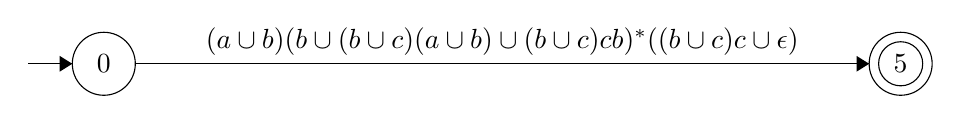
\begin{tikzpicture}[scale=0.2]
    \tikzstyle{every node}+=[inner sep=0pt]
    \draw [black] (5,-2.7) circle (2);
    \draw (5,-2.7) node {$0$};
    \draw [black] (55.6,-2.7) circle (2);
    \draw (55.6,-2.7) node {$5$};
    \draw [black] (55.6,-2.7) circle (1.4);
    \draw [black] (0.2,-2.7) -- (3,-2.7);
    \fill [black] (3,-2.7) -- (2.2,-2.2) -- (2.2,-3.2);
    \draw [black] (7,-2.7) -- (53.6,-2.7);
    \fill [black] (53.6,-2.7) -- (52.8,-2.2) -- (52.8,-3.2);
    \draw (30.3,-2.2) node [above] {$(a\cup b)(b\cup (b\cup c)(a\cup b)\cup (b\cup c)cb)^*((b\cup c)c\cup \epsilon)$};
    \end{tikzpicture}
\subcaption{After ripping \(2\).}
\end{subfigure}
\caption{Converting DFA to Regular Expression.}
\label{fig:automata3-2-2}
\end{figure}

\pagebreak
So the resulting regular expression is \((a\cup b)(b\cup (b\cup c)(a\cup b)\cup (b\cup c)cb)^*((b\cup c)c\cup \epsilon)\).
\subsection{}
\subsubsection{}
We know:
\begin{align}
\begin{rcases*}
x \in x^*\\
y \in yx^*
\end{rcases*}
\implies (x\cup y) \subseteq (x^*\cup yx^*) \implies (x\cup y)^* \subseteq (x^*\cup yx^*)^*
\end{align}
and also we know that \((x\cup y)^*\) is language of all strings of arbitrary length over the alphabet \(\{a, b\}\).
So:
\begin{align}
    (x^*\cup yx^*)^* \subseteq (x\cup y)^* 
\end{align}
Thus we have:
\begin{align}
    (x\cup y)^* = (x^*\cup yx^*)^*
\end{align}
\subsubsection{}
We use result of the last part:
\begin{align}
(y^*(x\cup \epsilon) y^*)^* &= (y^*xy^* \cup y^* y^*)^*\\
&= (y^*xy^* \cup y^*)^*\\
&= (y^* \cup y^*xy^*)^*\\
\xrightarrow{b = y, a = y^*x}&= (b^* \cup ab^*)^*\\
&= (b \cup a)^* & \text{using the last part}\\
&= (y \cup y^*x)^*
\end{align}
Again using the same reasoning as last part, we can get:
\begin{gather}
\begin{rcases*}
x \in y^*x \implies (y \cup x) \subseteq (y \cup y^*x) \implies (y \cup x)^* \subseteq (y \cup y^*x)^*\\
(y \cup y^*x)^* \subseteq \text{language of all strings over \(\{a, b\}\)} \implies (y \cup x)^* \subseteq (y \cup x)^*
\end{rcases*}\\
\implies (y^*(x\cup \epsilon) y^*)^* = (y \cup y^*x)^* = (y \cup x)^* = (x\cup y)^*
\end{gather}

\subsection{}
\subsubsection{}
We know that \(A\) generates strings of arbitrary length containing \(a\) (i.e. \(a^*\)).
So strings generated by \(S\) are of the form \(a^*(a^*ba^*b)^*b\).
And language of this regex can be described by the following NFA (Figure~\ref{fig:automata3-4-a}).
\begin{figure}[H]
\centering
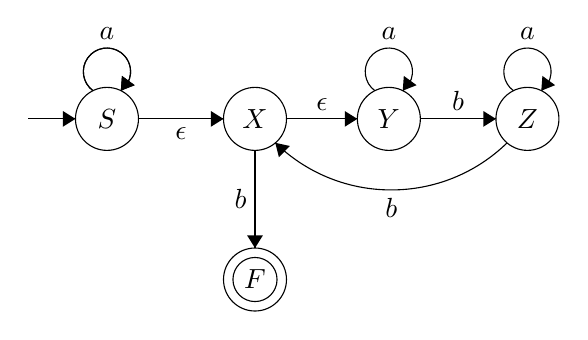
\begin{tikzpicture}[scale=0.2]
    \tikzstyle{every node}+=[inner sep=0pt]
    \draw [black] (5.2,-6.4) circle (2);
    \draw (5.2,-6.4) node {$S$};
    \draw [black] (14.6,-6.4) circle (2);
    \draw (14.6,-6.4) node {$X$};
    \draw [black] (14.6,-16.6) circle (2);
    \draw (14.6,-16.6) node {$F$};
    \draw [black] (14.6,-16.6) circle (1.4);
    \draw [black] (23.1,-6.4) circle (2);
    \draw (23.1,-6.4) node {$Y$};
    \draw [black] (31.9,-6.4) circle (2);
    \draw (31.9,-6.4) node {$Z$};
    \draw [black] (0.2,-6.4) -- (3.2,-6.4);
    \fill [black] (3.2,-6.4) -- (2.4,-5.9) -- (2.4,-6.9);
    \draw [black] (4.318,-4.614) arc (234:-54:1.5);
    \draw (5.2,-1.4) node [above] {$a$};
    \fill [black] (6.08,-4.61) -- (6.96,-4.26) -- (6.15,-3.67);
    \draw [black] (4.318,-4.614) arc (234:-54:1.5);
    \fill [black] (6.08,-4.61) -- (6.96,-4.26) -- (6.15,-3.67);
    \draw [black] (7.2,-6.4) -- (12.6,-6.4);
    \fill [black] (12.6,-6.4) -- (11.8,-5.9) -- (11.8,-6.9);
    \draw (9.9,-6.9) node [below] {$\epsilon$};
    \draw [black] (14.6,-8.4) -- (14.6,-14.6);
    \fill [black] (14.6,-14.6) -- (15.1,-13.8) -- (14.1,-13.8);
    \draw (14.1,-11.5) node [left] {$b$};
    \draw [black] (16.6,-6.4) -- (21.1,-6.4);
    \fill [black] (21.1,-6.4) -- (20.3,-5.9) -- (20.3,-6.9);
    \draw (18.85,-5.9) node [above] {$\epsilon$};
    \draw [black] (22.218,-4.614) arc (234:-54:1.5);
    \draw (23.1,-1.4) node [above] {$a$};
    \fill [black] (23.98,-4.61) -- (24.86,-4.26) -- (24.05,-3.67);
    \draw [black] (25.1,-6.4) -- (29.9,-6.4);
    \fill [black] (29.9,-6.4) -- (29.1,-5.9) -- (29.1,-6.9);
    \draw (27.5,-5.9) node [above] {$b$};
    \draw [black] (31.018,-4.614) arc (234:-54:1.5);
    \draw (31.9,-1.4) node [above] {$a$};
    \fill [black] (32.78,-4.61) -- (33.66,-4.26) -- (32.85,-3.67);
    \draw [black] (30.608,-7.922) arc (-45.75798:-134.24202:10.546);
    \fill [black] (15.89,-7.92) -- (16.12,-8.84) -- (16.81,-8.12);
    \draw (23.25,-11.41) node [below] {$b$};
    \end{tikzpicture}
\caption{DFA for the regex \(a^*(a^*ba^*b)^*b\).}
\label{fig:automata3-4-a}
\end{figure}
And we can convert this NFA to a left-linear grammar easily.
\begin{equation}
\begin{aligned}
    S &\rightarrow aS \mid X\\
    X &\rightarrow Y \mid b\\
    Y &\rightarrow aY \mid bZ\\
    Z &\rightarrow  aZ \mid b X
\end{aligned}
\end{equation}

\subsubsection{}
If we examine this grammar carefully, we can see that it describes language of strings with even number of \(a\)s (because either \(S\Rightarrow B\) and \(S\) has no \(a\)s, or \(S\Rightarrow AA\), where each time using \(A\to AAA\) rule, adds 2 \(a\)s to the string).
So we can design the following DFA (Figure~\ref{fig:automata3-4-b}) to recognize this language.
\begin{figure}[H]
\centering
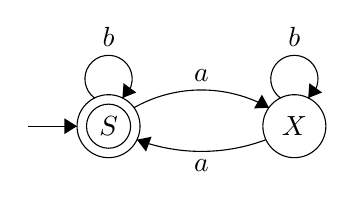
\begin{tikzpicture}[scale=0.2]
    \tikzstyle{every node}+=[inner sep=0pt]
    \draw [black] (5.3,-6.9) circle (2);
    \draw (5.3,-6.9) node {$S$};
    \draw [black] (5.3,-6.9) circle (1.4);
    \draw [black] (17.1,-6.9) circle (2);
    \draw (17.1,-6.9) node {$X$};
    \draw [black] (0.2,-6.9) -- (3.3,-6.9);
    \fill [black] (3.3,-6.9) -- (2.5,-6.4) -- (2.5,-7.4);
    \draw [black] (6.914,-5.726) arc (119.44954:60.55046:8.717);
    \fill [black] (15.49,-5.73) -- (15.04,-4.9) -- (14.54,-5.77);
    \draw (11.2,-4.1) node [above] {$a$};
    \draw [black] (15.297,-7.759) arc (-69.44472:-110.55528:11.667);
    \fill [black] (7.1,-7.76) -- (7.68,-8.51) -- (8.03,-7.57);
    \draw (11.2,-9) node [below] {$a$};
    \draw [black] (16.218,-5.114) arc (234:-54:1.5);
    \draw (17.1,-1.9) node [above] {$b$};
    \fill [black] (17.98,-5.11) -- (18.86,-4.76) -- (18.05,-4.17);
    \draw [black] (4.418,-5.114) arc (234:-54:1.5);
    \draw (5.3,-1.9) node [above] {$b$};
    \fill [black] (6.18,-5.11) -- (7.06,-4.76) -- (6.25,-4.17);
    \end{tikzpicture}
\caption{DFA for the language of strings with even number of \(a\)s.}
\label{fig:automata3-4-b}
\end{figure}
The equivalent left-linear grammar is:
\begin{equation}
\begin{aligned}
S &\rightarrow bS \mid aX \mid \epsilon\\    
X &\rightarrow bX \mid aS
\end{aligned}
\end{equation}

\section{Closure Properties of Regular Languages}
\subsection{}
We design a NFA which recognizes the language of \(\putx(L, x)\) (i.e., \(D_2\)) using the NFA of \(L\) (i.e., \(D\)).
The main idea is to duplicate every state and transition of \(D\) and add a new transition from every state of \(D\) to their corresponding duplicate state, accepting the input \(x\)
(for brevity, here we assume that our new transitions can input a string of arbitrary length, instead of a single character).
And finally, only the duplicate of the final state of \(D\) will be accepting states.
Doing so, we the read inputs and proceed in the initial NFA, \(D\).
As soon as \(x\) is read, we switch to the duplicate of the current state and proceed in the duplicate NFA until we reach its final state.
We can show this procedure formally as follows:
\begin{align}
D = (Q, \Sigma, \delta, q_0, F)
\end{align}
We denote the corresponding state of \(q\) as \(q'\).
\begin{align}
D_2 = (Q_2, \Sigma, \delta_2, q_0, F')
\end{align}
where:
\begin{gather}
Q' \triangleq \bigcup_{q \in Q} \{q'\} \quad \text{and} \quad F' \triangleq \bigcup_{q \in F}\{q'\}\\
Q_2 = Q \cup Q'\\
\delta_2(s, a) =
\begin{cases}
\delta(q, a) & \text{if } s=q \in Q \text{ and \(a\neq x\)}\\
\delta(q, a)\cup \{q'\} & \text{if } s=q \in Q \text{ and \(a=x\)}\\
\delta'(q, a)  & \text{if } s=q' \in Q'
\end{cases}
\end{gather}
Clarifying using an example: \(L=\) all strings over \(\{a, b\}\) with even number of \(a\)s.
\begin{figure}[H]
\centering
\begin{subfigure}[]{0.45\textwidth}
\centering
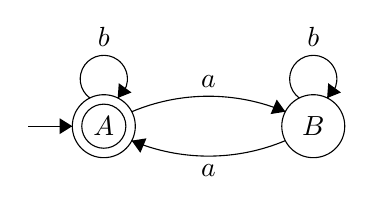
\begin{tikzpicture}[scale=0.2]
    \tikzstyle{every node}+=[inner sep=0pt]
    \draw [black] (18.3,-6.9) circle (2);
    \draw (18.3,-6.9) node {$B$};
    \draw [black] (5,-6.9) circle (2);
    \draw (5,-6.9) node {$A$};
    \draw [black] (5,-6.9) circle (1.4);
    \draw [black] (4.118,-5.114) arc (234:-54:1.5);
    \draw (5,-1.9) node [above] {$b$};
    \fill [black] (5.88,-5.11) -- (6.76,-4.76) -- (5.95,-4.17);
    \draw [black] (17.418,-5.114) arc (234:-54:1.5);
    \draw (18.3,-1.9) node [above] {$b$};
    \fill [black] (19.18,-5.11) -- (20.06,-4.76) -- (19.25,-4.17);
    \draw [black] (6.774,-5.981) arc (112.81668:67.18332:12.574);
    \fill [black] (16.53,-5.98) -- (15.98,-5.21) -- (15.59,-6.13);
    \draw (11.65,-4.5) node [above] {$a$};
    \draw [black] (16.525,-7.818) arc (-67.2022:-112.7978:12.582);
    \fill [black] (6.77,-7.82) -- (7.32,-8.59) -- (7.71,-7.67);
    \draw (11.65,-9.3) node [below] {$a$};
    \draw [black] (0.2,-6.9) -- (3,-6.9);
    \fill [black] (3,-6.9) -- (2.2,-6.4) -- (2.2,-7.4);
    \end{tikzpicture}
\caption{\(D\).}
\label{fig:automata4-1}
\end{subfigure}
\(\implies\)
\begin{subfigure}[]{0.45\textwidth}
\centering
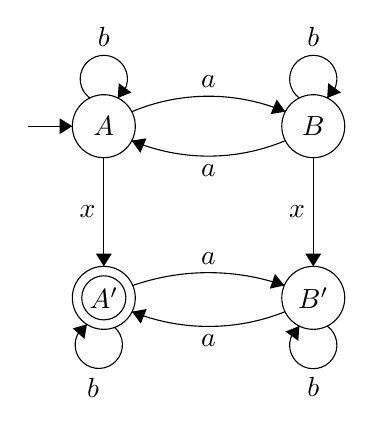
\begin{tikzpicture}[scale=0.2]
    \tikzstyle{every node}+=[inner sep=0pt]
    \draw [black] (18.3,-6.9) circle (2);
    \draw (18.3,-6.9) node {$B$};
    \draw [black] (5,-6.9) circle (2);
    \draw (5,-6.9) node {$A$};
    \draw [black] (5,-17.8) circle (2);
    \draw (5,-17.8) node {$A'$};
    \draw [black] (5,-17.8) circle (1.4);
    \draw [black] (18.3,-17.8) circle (2);
    \draw (18.3,-17.8) node {$B'$};
    \draw [black] (4.118,-5.114) arc (234:-54:1.5);
    \draw (5,-1.9) node [above] {$b$};
    \fill [black] (5.88,-5.11) -- (6.76,-4.76) -- (5.95,-4.17);
    \draw [black] (17.418,-5.114) arc (234:-54:1.5);
    \draw (18.3,-1.9) node [above] {$b$};
    \fill [black] (19.18,-5.11) -- (20.06,-4.76) -- (19.25,-4.17);
    \draw [black] (6.774,-5.981) arc (112.81668:67.18332:12.574);
    \fill [black] (16.53,-5.98) -- (15.98,-5.21) -- (15.59,-6.13);
    \draw (11.65,-4.5) node [above] {$a$};
    \draw [black] (16.525,-7.818) arc (-67.2022:-112.7978:12.582);
    \fill [black] (6.77,-7.82) -- (7.32,-8.59) -- (7.71,-7.67);
    \draw (11.65,-9.3) node [below] {$a$};
    \draw [black] (5,-8.9) -- (5,-15.8);
    \fill [black] (5,-15.8) -- (5.5,-15) -- (4.5,-15);
    \draw (4.5,-12.35) node [left] {$x$};
    \draw [black] (18.3,-8.9) -- (18.3,-15.8);
    \fill [black] (18.3,-15.8) -- (18.8,-15) -- (17.8,-15);
    \draw (17.8,-12.35) node [left] {$x$};
    \draw [black] (6.838,-17.015) arc (109.2194:70.7806:14.619);
    \fill [black] (16.46,-17.01) -- (15.87,-16.28) -- (15.54,-17.22);
    \draw (11.65,-15.7) node [above] {$a$};
    \draw [black] (16.507,-18.681) arc (-68.20827:-111.79173:13.083);
    \fill [black] (6.79,-18.68) -- (7.35,-19.44) -- (7.72,-18.51);
    \draw (11.65,-20.12) node [below] {$a$};
    \draw [black] (5.687,-19.67) arc (47.90571:-240.09429:1.5);
    \draw (4.31,-22.86) node [below] {$b$};
    \fill [black] (3.93,-19.48) -- (3.03,-19.74) -- (3.77,-20.41);
    \draw [black] (0.2,-6.9) -- (3,-6.9);
    \fill [black] (3,-6.9) -- (2.2,-6.4) -- (2.2,-7.4);
    \draw [black] (19.182,-19.586) arc (54:-234:1.5);
    \draw (18.3,-22.8) node [below] {$b$};
    \fill [black] (17.42,-19.59) -- (16.54,-19.94) -- (17.35,-20.53);
    \end{tikzpicture}
\caption{\(D_2\).}
\label{fig:automata4-1-b}
\end{subfigure}
\end{figure}
And \(D_2\) describes \(\putx(L, x)\).

\subsection{}
We will first solve part~\ref{sec:subsubsection4-2}.
\setsubsubsectionnumber{2}
\subsubsection{}\label{sec:subsubsection4-2}
We want to prove that if \(L\) is a regular language, \(\textup{SQRT}(L) = \left\{x \mid \exists y:\ \abs{y}=\abs{x}^2, xy\in L\right\}\) is a regular language.\\
Assume the DFA recognizing \(L\) is \(D = (Q, \Sigma, \delta, q_0, F)\).\\
We define \(\mathcal{G}\) to be the set of all functions from \(Q\) to \(\mathcal{P}(Q)\) (power-set of \(Q\)). 
And for any \(f, g \in \mathcal{G}\), we define \(f \circ g\) as follows:
\begin{align}
f \circ g(q) = \bigcup_{q' \in g(q)} f(q')
\end{align}
Construct the new DFA \(D'\) recognizing \(\textup{SQRT}(L)\) as follows:
\begin{align}
D' &= (Q', \Sigma, \delta', q_0', F')\\
Q' &= Q \times \mathcal{G}^2\\
\delta'((q, g_1, g_2), a) &= \Big(\delta(q, a), g_1\circ g_0, ((g_2\circ g_1)\circ g_1)\circ g_0\Big)\\
\text{Where }g_0(q) &= \left\{\delta(q, a)\mid a \in \Sigma\right\}\\
q_0' &= (q_0, I, I)\\
\text{Where }I(q) &= \left\{q\right\}\\
F' &= \left\{(q, g_1, g_2) \in Q\times \mathcal{G}^2 \mid g_2(q) \cap F \neq \emptyset\right\}
\end{align}
In this new DFA, after reading a word \(w\), if \(D\) reaches state \(q\), then \(D'\) reaches the state \((q, g_1, g_2)\) where \(g_1(.)\) and \(g_2(.)\) represent the set of states of \(D\) that can be reached starting at \(.\) then reading a string of length \(\abs{w}\) and \(\abs{w}^2\) respectively.
This can be proved using induction on strings of length \(n\).
When \(n=0\) (no character is read), \(g_1(.)\) and \(g_2(.)\) are contain only \(.\) state.\\
If our claim holds for strings of length \(n=k\), we have:
\begin{align}
\delta'(q_0', w) &= (q, g_1, g_2) \tab \forall w: \abs{w}=k\\
g_1(.) &= \left\{\text{all states reachable from \(.\) with \(k\) steps}\right\}\\
g_2(.) &= \left\{\text{all states reachable from \(.\) with \(k^2\) steps}\right\}\\
g_0(.) &= \left\{\delta(. , a)\mid a \in \Sigma\right\}\\
\implies g_0(.) & = \left\{\text{all states reachable from \(.\) with \(1\) step}\right\}\\
\text{Now for \(n=k+1\), we have:}\tag*{}\\
\forall a \in \Sigma: \delta'((q, g_1, g_2), a) &= \Big(\delta(q, a), g_1\circ g_0, ((g_2\circ g_1)\circ g_1)\circ g_0\Big)\\
\implies g_1\circ g_0(.) &= \left\{\text{all states reachable from \(.\) with \(k+1\) steps}\right\}\\
\text{and } ((g_2\circ g_1)\circ g_1)\circ g_0 &= \{\text{all states reachable from \(.\) with \(\underbrace{k^2 + k + k + 1}_{=(k+1)^2}\) steps}\}
\end{align}
Thus we have proved our claim.
And we have designed a DFA \(D'\) recognizing \(\textup{SQRT}(L)\).
So \(\textup{SQRT}(L)\) is a regular language.

\setsubsubsectionnumber{1}
\subsubsection{}
A similar argument can be used to prove this part.
This time we use functions in \(\mathcal{G}\) to keep track of length of strings in \(B\).
\begin{align}
A, B \text{ are regular} \implies \textup{C}(A, B) = \left\{x\in A \mid \exists y:\ \abs{y}=\abs{x}^2, y \in B \right\} \text{ is regular}
\end{align}
There exists DFAs \(D_A\) and \(D_B\) recognizing \(A\) and \(B\) respectively.
We design a DFA \(D_C\) recognizing \(\textup{C}(A, B)\) as follows:
\begin{align}
D_A &= (Q_A, \Sigma, \delta_A, q_{0, A}, F_A)\\
D_B &= (Q_B, \Sigma, \delta_B, q_{0, B}, F_B)\\
D_C &= (Q_C, \Sigma, \delta_C, q_{0, C}, F_C)\\
\text{Where: }Q_C &= Q_A \times \mathcal{G}^2\\
\delta_C((q, g_1, g_2), a) &= \Big(\delta_A(q, a), g_1\circ g_0, ((g_2\circ g_1)\circ g_1)\circ g_0\Big)\\
\text{Where }g_0(.) &= \left\{\delta_B(q, .)\mid a \in \Sigma\right\}\\
q_{0, C} &= (q_{0, A}, I, I)\\
\text{Where }I(.) &= \left\{.\right\}\\
F_C &= \left\{(q, g_1, g_2) \in Q_A\times \mathcal{G}^2 \mid q\in F_A \text{ and } g_2(q_{0,B}) \cap F_B \neq \emptyset\right\}
\end{align}

\section{Proving Non-Regularity of Languages}
\subsection{}
\subsubsection{}
Proof by contradiction.
Assume \(L_1\) is a regular language and its pumping length is \(p\).
Consider the string \(w = a^pb^{p!+p}c^{p!+p}\).
Because \(w\) is a member of \(L_1\) and has length more than \(p\), the pumping lemma guarantees that \(w\) can be split into three pieces, \(w = xyz\), satisfying the lemma conditions.
We know that \(\vert xy\vert \le p\) and \(\vert y\vert \ge 1\).
So \(x\) and \(y\) contain only \(a\)s.
Pumping this strings we get:
\begin{gather}
xy^iz \in L_1 \quad \text{for all } i \in \mathbb{N}.
\end{gather}
If we take \(y\)'s length to be \(k\), number of \(a\)s in \(xy^iz\) will be \(p-k+ki\).
And we can find an \(i\) such that the number of \(a\)s, \(b\)s, and \(c\)s are equal in \(xy^iz\).
\begin{align}
&p - k + ki = p! + p\\
\implies & k(i-1) = p!\\
\xrightarrow{k \le p \implies k|p!} & i = \frac{p!}{k}+1
\end{align}
So the string \(a^{p!+p}b^{p!+p}c^{p!+p}\) can be achieved by pumping \(a^pb^{p!+p}c^{p!+p}\), but it is not a member of \(L_1\).
So we have reached a contradiction and \(L_1\) is not a regular language.

\subsubsection{}
Assume \(L_2\) is a regular language, \(p\) is its pumping length and \(r\) is the smallest prime number such that \(p \le r\).
Consider the string \(a^{2r}\).
The pumping lemma guarantees that this string can be split into three pieces, \(a^{2r} = xyz\), satisfying the lemma conditions.
Assuming \(y\)'s length to be \(k\), we have:
\begin{align}
\abs{xy^iz} = 2r - k + ik = 2r + (i-1)k \text{ is product of two prime numbers.}
\end{align}
For odd values of \(i\) we have:
\begin{align}
&i = 2j + 1\\
\implies & 2r + (2j)k = 2(r + jk) \text{ is product of two prime numbers.}\\
\implies & r + jk \text{ is a prime number.}
\end{align}
So we have a linear pattern for generating prime numbers larger than \(r\)!
And we know that there is no such pattern.
So we have reached a contradiction and \(L_2\) is not a regular language.

\subsection{To Do}

\end{document}